\documentclass{beamer}
\usepackage{beamerthemeshadow}
\usepackage[utf8]{inputenc}  
\usepackage{longtable}
\usepackage{minted}
\usepackage[ngermanb]{babel}
\beamersetuncovermixins{\opaqueness<1>{25}}{\opaqueness<2->{15}}
\setbeamertemplate{navigation symbols}{}%remove navigation symbols
\begin{document}

% Latex Beamer Übersicht: 
% https://www2.informatik.hu-berlin.de/~mischulz/beamer.html

\title{WebPiraten}  
\author{A. Flohr, C. Nehls, M. Rasch,  M. Neumann}
\date{22.08.2014} 

\begin{frame}
\maketitle
\end{frame} 

%\begin{frame}
%\frametitle{Inhalt}
%\tableofcontents
%\end{frame}

%\begin{frame}
%\begin{itemize}
%\item Demo
%\item Übersichtgrafik
%\item Use-Case (grob)\newline
%-$>$ GUI -(websocket)-$>$ Preprocossor -(TCP)-$>$ VM -(STDIN)-$>$ Ausführung -(STDIN)-$>$ %VM-Wrapper -(TCP)-$>$ Rails-Simulation -(websocket)-$>$ GUI $<$-
%\item Preprocessor
%\item VM
%\item Simulation
%\item Client
%\item Erlang
%\item Scopes
%\item Sicherheit
%\item Performance
%\end{itemize}
%\end{frame}

\section{Die WebApp}

\section{Use-Case}

\section{Module}
\subsection{Präprozesssor für Ruby}

\begin{frame}
\begin{center}
	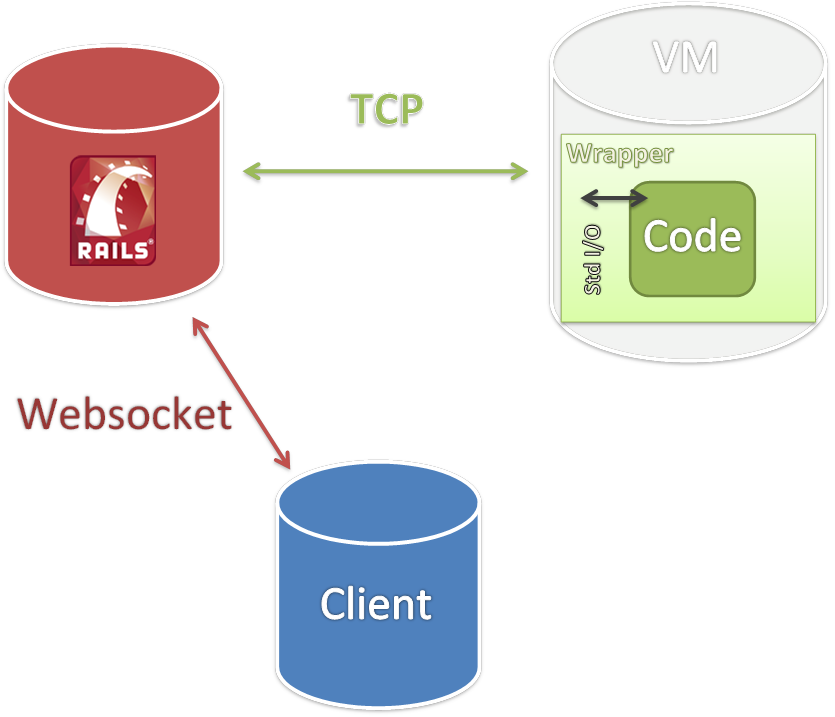
\includegraphics[scale=0.35]{overview}
\end{center}
\end{frame}

\begin{frame}
\frametitle{Idee}
%Ruby, rub, rub! :3
\begin{center}
\includegraphics[scale=0.5]{preprocessor/pics/Idee}
\end{center}
%Spiellogik vor den User code kopieren und den Code für das line highlighting und das Verfolgen von Variablen mit dem nötigen Input füttern.
\end{frame}

\begin{frame}
\frametitle{Erkennung von Sonderfällen}
	\includegraphics[scale=0.70]{preprocessor/pics/CodeArten}
\end{frame}

\begin{frame}
\frametitle{Standard Verfahren}
\inputminted[linenos, numbersep=3pt, tabsize=2, frame=lines]{ruby}{preprocessor/sampleStandard.rb}
\end{frame}

\begin{frame}
\frametitle{Standard Verfahren mit Variablenverfolgung}
  \inputminted[linenos, numbersep=5pt, tabsize=4, frame=lines]{ruby}{preprocessor/sampleDebug.rb}
\end{frame}

\begin{frame}
\frametitle{Verarbeitung mehrzeiliger Strings}
  \includegraphics[scale=1]{preprocessor/pics/MultilineVerarbeitung}
\end{frame}

%\begin{frame}
%\frametitle{Verarbeitung von Case Blöcken}
%\begin{center}
%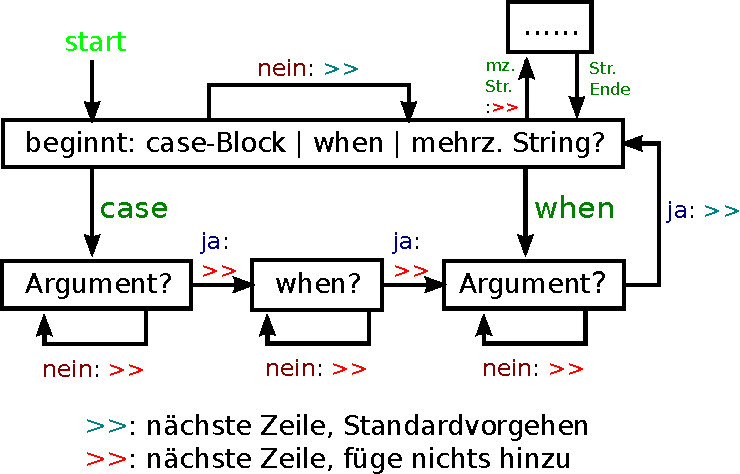
\includegraphics[scale=0.8]{preprocessor/pics/CaseBlockVerarbeitung}
%\end{center}
%\end{frame}

\begin{frame}
%\frametitle{Code: vorher und nachher}
  \begin{columns}
    \column[t]{0.50\textwidth}
\inputminted[linenos, frame=lines, tabsize=2, fontsize=\footnotesize , label=case when einzeilig]{ruby}{preprocessor/CaseB.rb}
    \column[t]{0.50\textwidth}
    \inputminted[linenos, frame=lines, tabsize=2, fontsize=\footnotesize , label=case mehrzeilig]{ruby}{preprocessor/CaseA.rb}
  \end{columns} 
\end{frame}

\begin{frame}
%\frametitle{Code: vorher und nachher}
  \begin{columns}
    \column[t]{.50\textwidth}
\inputminted[ tabsize=2, fontsize=\footnotesize , label=vorher]{ruby}{preprocessor/sampleA.rb}
    \column[t]{.50\textwidth}
    \inputminted[ tabsize=2, fontsize=\footnotesize , label=danach]{ruby}{preprocessor/sampleB.rb}
  \end{columns} 
\end{frame}

\begin{frame}
\frametitle{Beschränkungen für den Nutzer}
  \begin{columns}
    \column[c]{.65\textwidth}
    \begin{itemize}
    \item \textit{return} bei eigenen Funktionen
    \item keine mehrzeiligen Strings der Form             
    \%q[Text des Strings] oder 
    
    \%Q[anderer Text]
    \end{itemize}
    \column[c]{.35\textwidth}
  
\includegraphics[scale=0.15]{preprocessor/pics/Verbotsschild}
  \end{columns} 
\end{frame}
\subsection{Codeausführung}

\begin{frame}
\begin{center}
	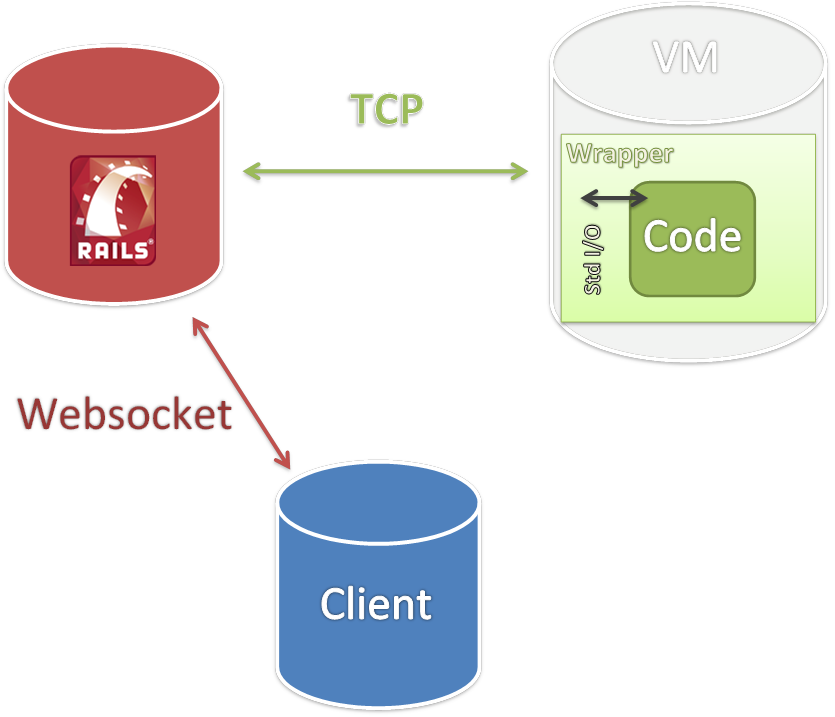
\includegraphics[scale=0.35]{overview}
\end{center}
\end{frame}

\begin{frame}
\frametitle{API}
\inputminted[linenos, numbersep=2pt, tabsize=4, frame=lines, label=move]{ruby}{vm/move.rb}
\end{frame}

\begin{frame}
\frametitle{API}
\inputminted[linenos, numbersep=2pt, tabsize=4, frame=lines, label=look]{ruby}{vm/look.rb}
\inputminted[linenos, numbersep=2pt, tabsize=4, frame=lines, label=response]{ruby}{vm/look_response.rb}
\end{frame}

\begin{frame}
\frametitle{Kommunikation mit der VM}
\begin{center}
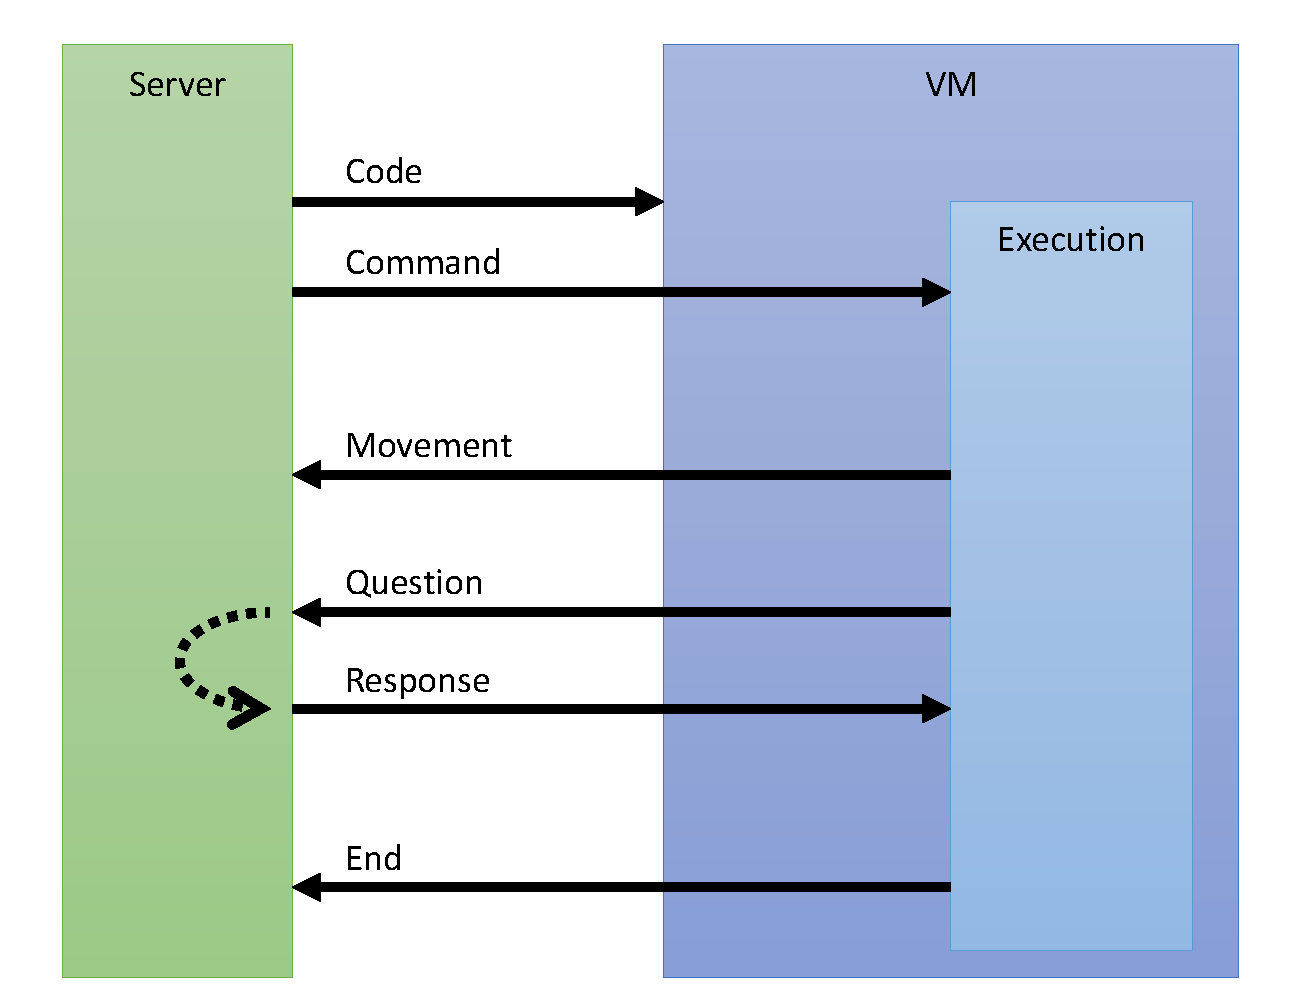
\includegraphics[width=250pt]{vm/vm.pdf}
\end{center}
\end{frame}
%\subsection{Simulation}




\begin{frame}
\begin{center}
	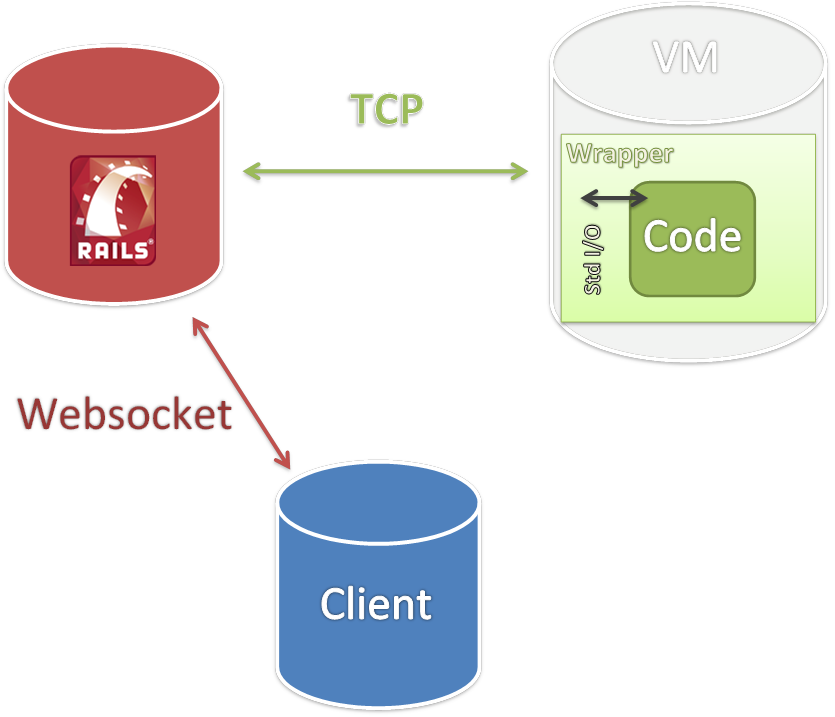
\includegraphics[scale=0.35]{overview}
\end{center}
\end{frame}



\begin{frame}
	\frametitle{History}
	\begin{center}
		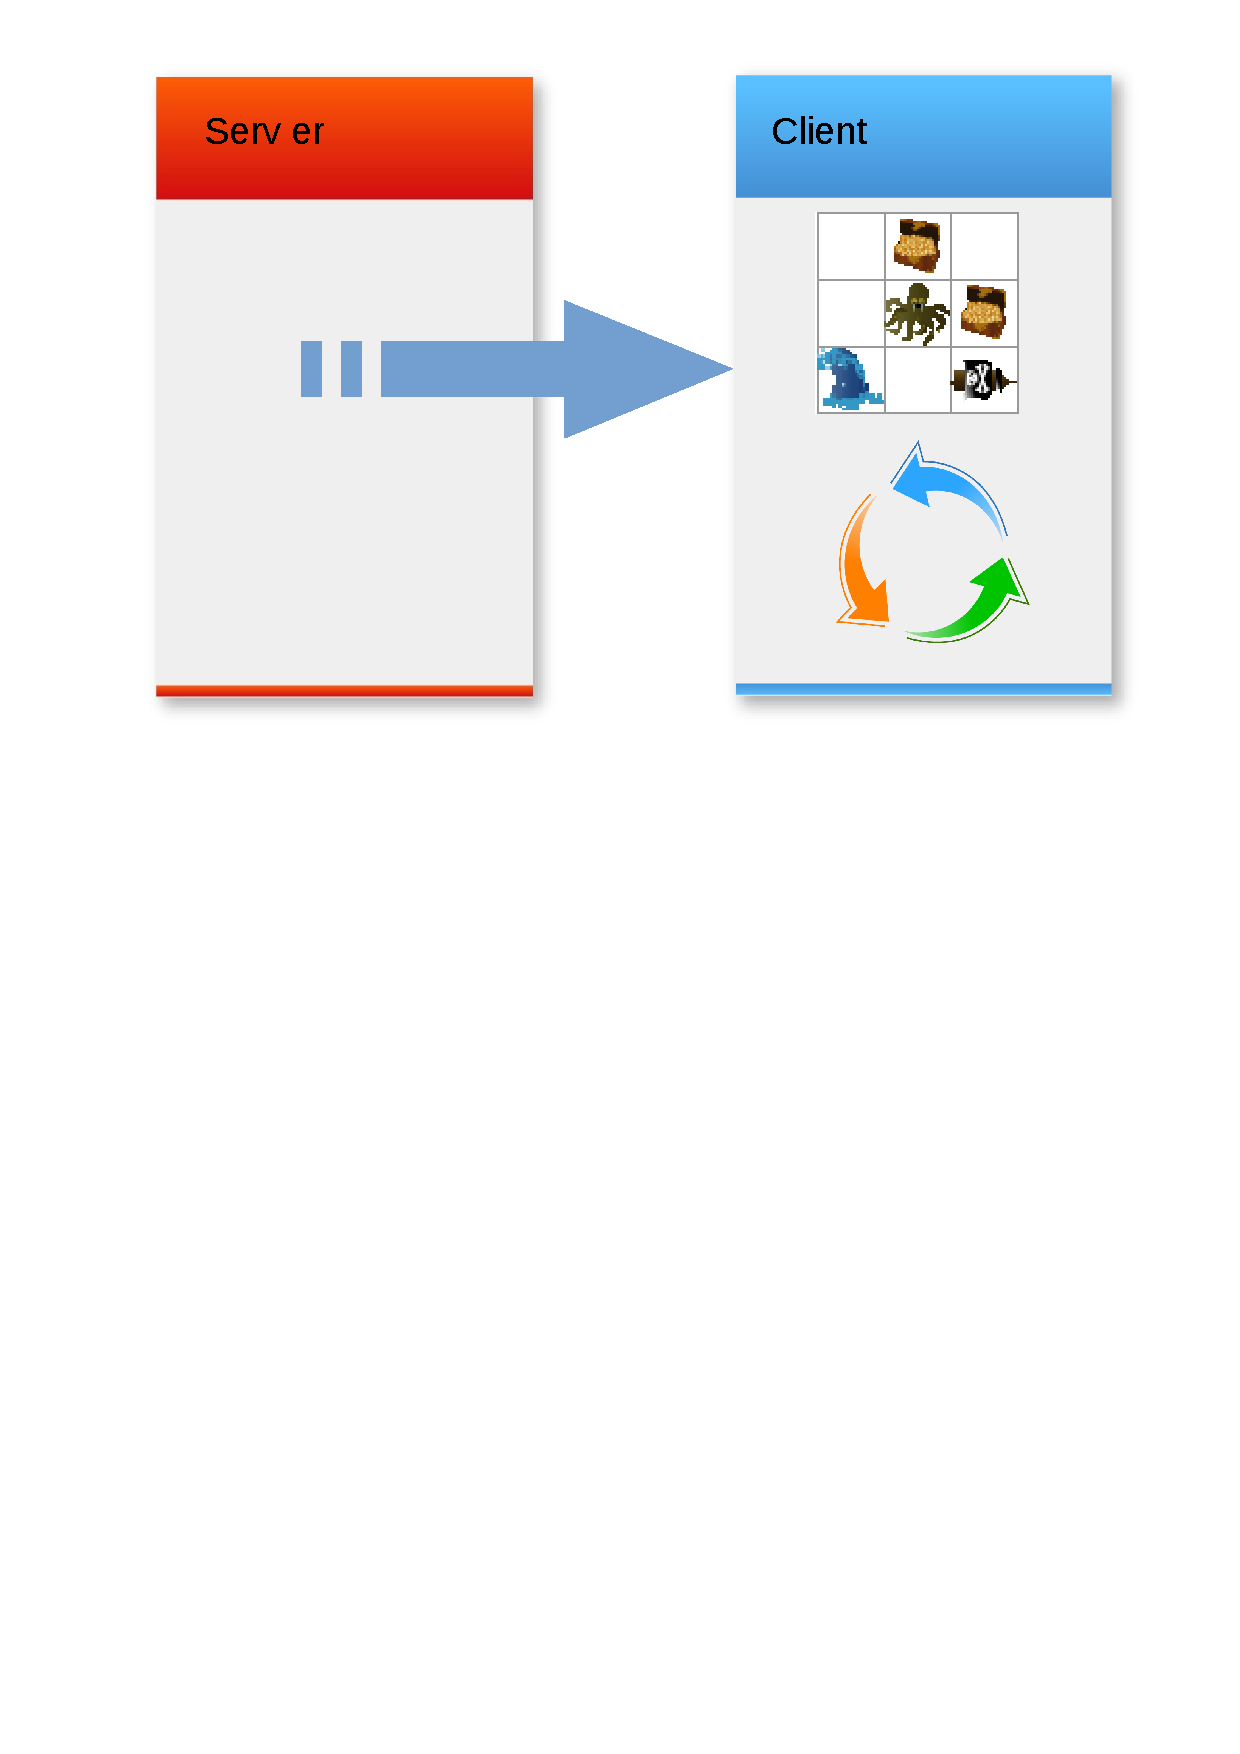
\includegraphics[scale=0.5]{simulation/history1.pdf}
	\end{center}
	%Wir haben ganz am Anfang ohne VM angefangen. Es gab zwei Ansätze, endweder die Simulation etc. auf dem Server oder auf dem Client. Der erste Entwurf sah vor, dass wir auf dem Client den eingegebenen Code zu Javascript compilieren und dann auf dem Client simulieren. Es traten viele Probleme mit dem compilieren auf, also entschlossen wir uns recht früh für eine VM.
\end{frame}

\begin{frame}
	\frametitle{History}
	\begin{center}
		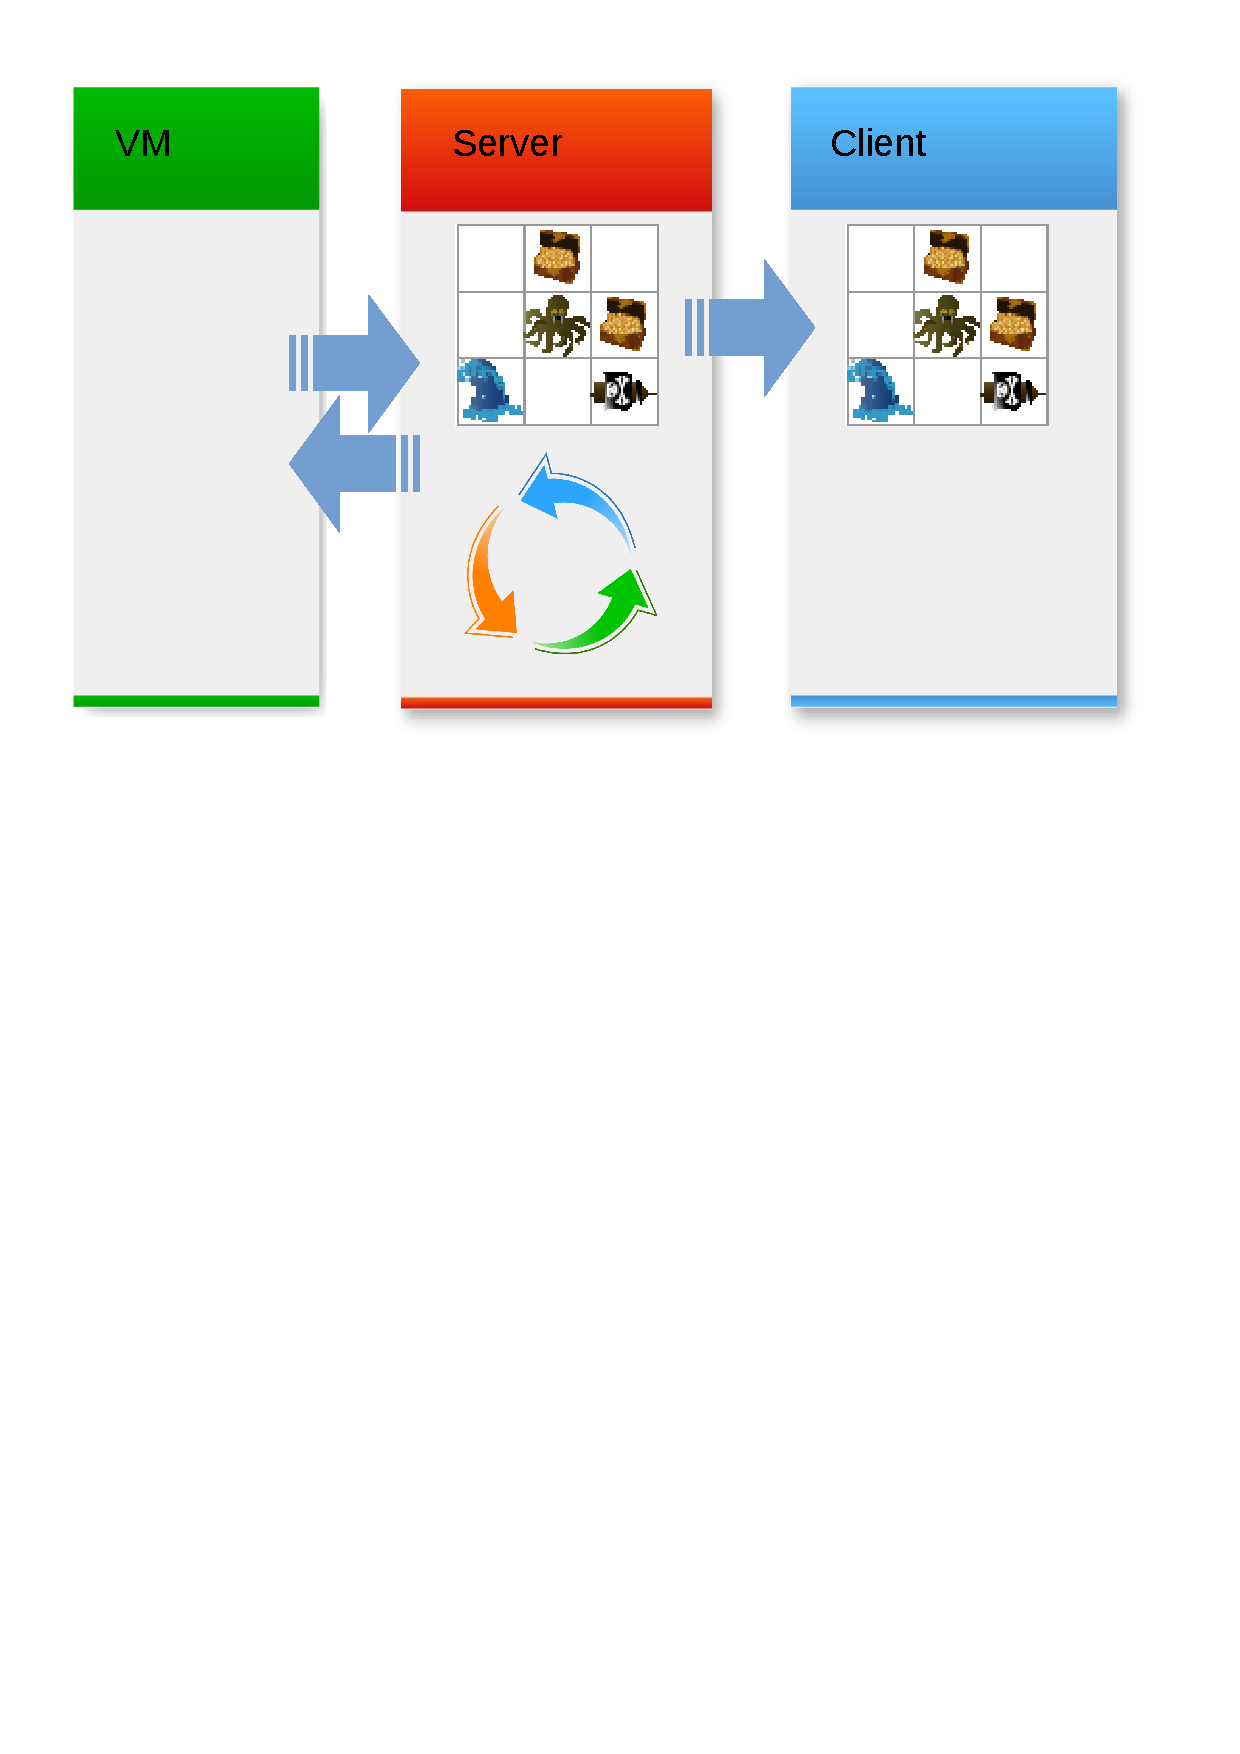
\includegraphics[scale=0.5]{simulation/history2.pdf}
	\end{center}
	%Am Anfang leitete der Server die Ausgaben der VM nur an den Client weiter, dies funktionierte prima, bis wir an den Punkt kamen, dass die VM auch Anfragen stellen konnte und dann wurde es sehr unpraktisch, immer auf Antwort vom Client zu warten. Wir haben das jetzt so gelöst, dass die Simulation quasi komplett auf dem Server läuft und nur die Änderungen des Grids an den Client weitergegeben werden.
\end{frame}


%jetzt geh ich noch ein paar schritte zurück und erkläre, wie wir angefangen haben.

\begin{frame}
	\begin{center}
		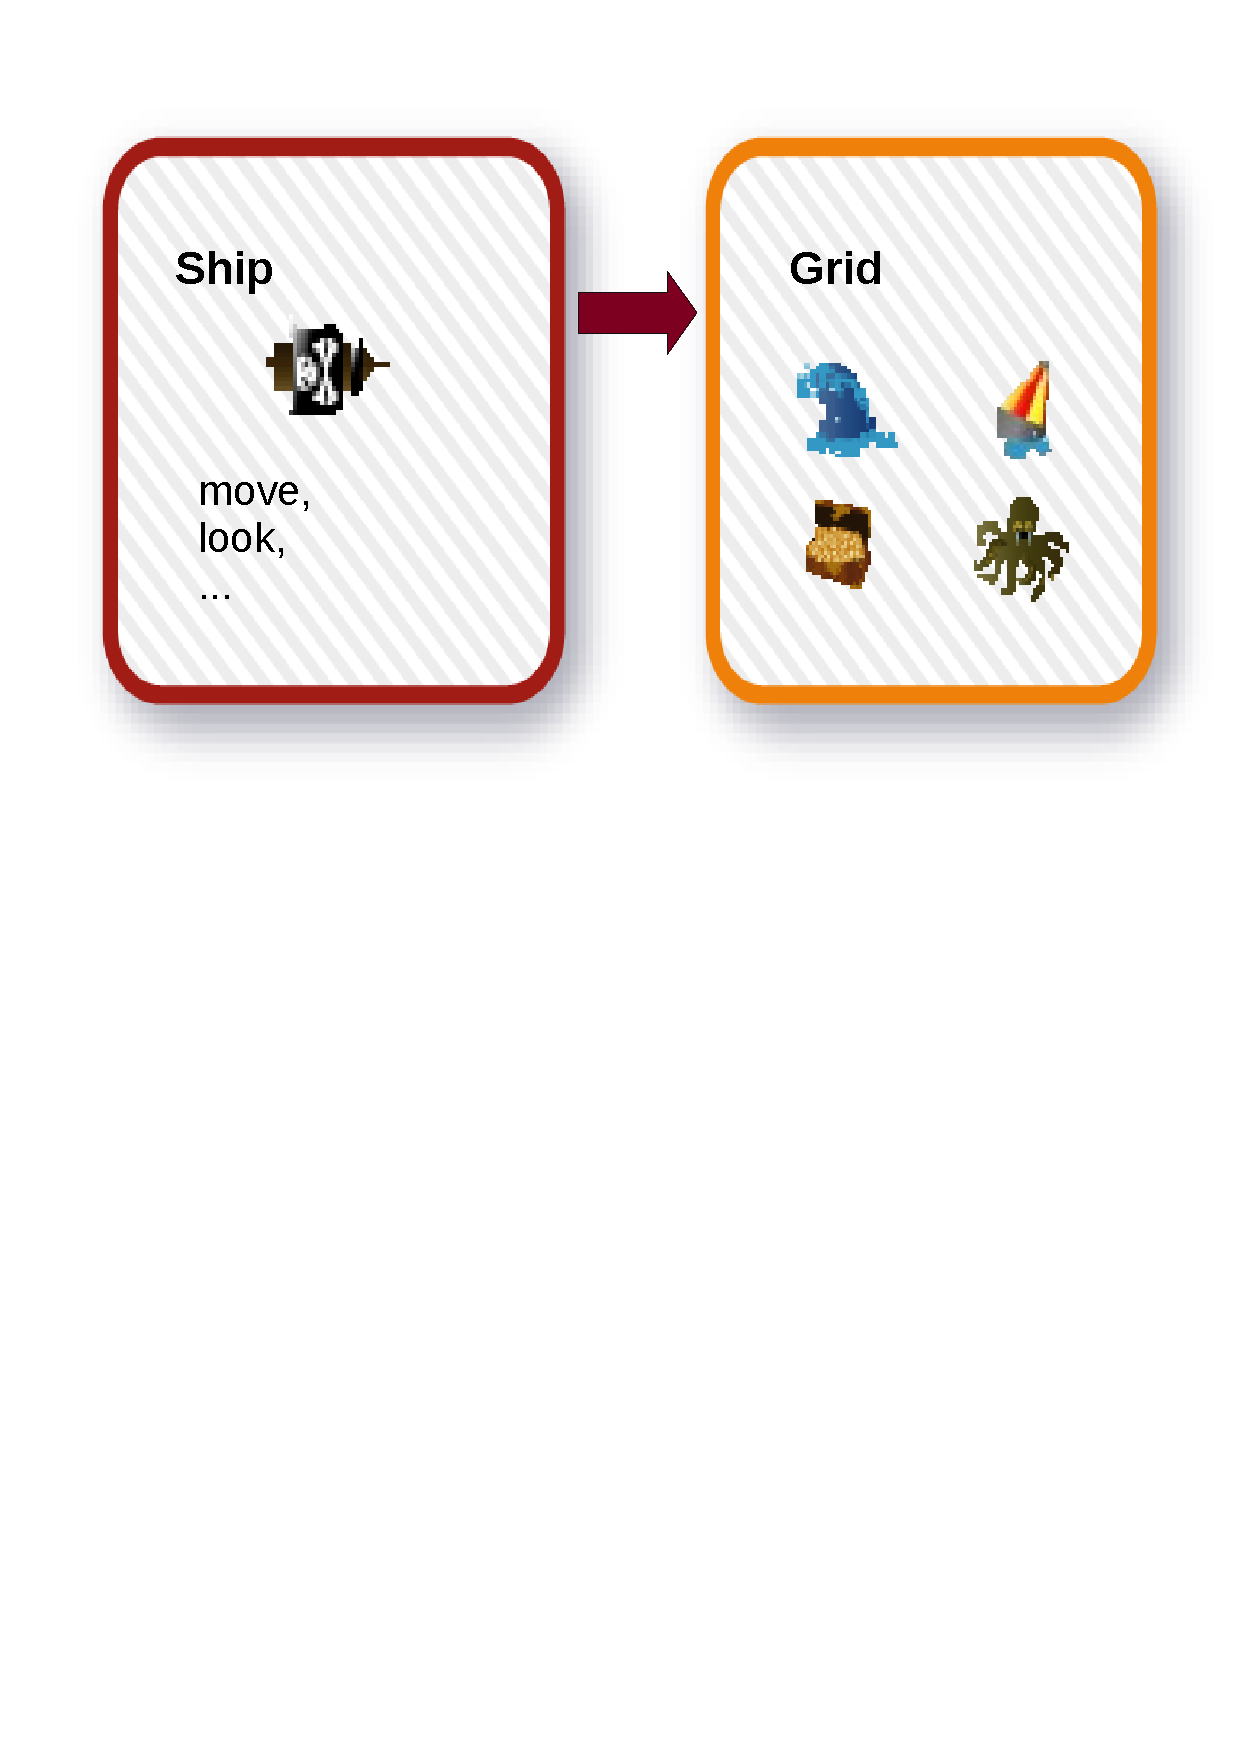
\includegraphics[scale=0.5]{simulation/Simulation6.pdf}
	\end{center}
	%Die Simulation ist der aktuelle Zustand des Systems. wir die aufteilung in Grid und Ship. Im Grid liegen nur die Objekte auf unserem Spielfeld unter ihren Koordinaten gespeichert. Die Ausführung ist stehts aus Sicht des Schiffes. Hier haben wir die ganzen Funktionen. Wir lesen die Ausgaben der VM aus und rufen die entsprechenden Funktionen auf. Dadurch ist die Simulation komplett Sprachunabhängig. Aus der Simulation können wir die VM stoppen und schicken alle wichtigen Daten per Paket an die GUI. 
\end{frame}

\begin{frame}
	\begin{center}
		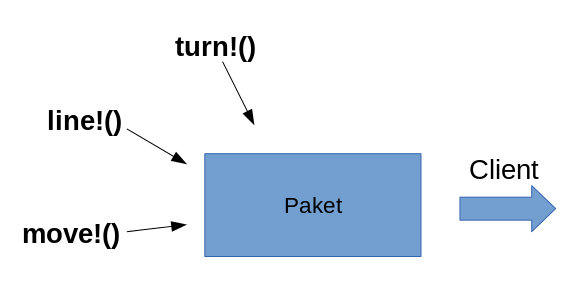
\includegraphics[scale=0.5]{simulation/Pakete.jpg}
	\end{center}
	%Für jede Zeile des ursprünglichen Codes wird ein Paket gepackt, in die jede aufgerufene Funktion Informationen für den Server packen können. Ist man am Ende einer Zeile angelangt, wird das Paket losgeschickt. 
\end{frame}


\begin{frame}
	\begin{center}
		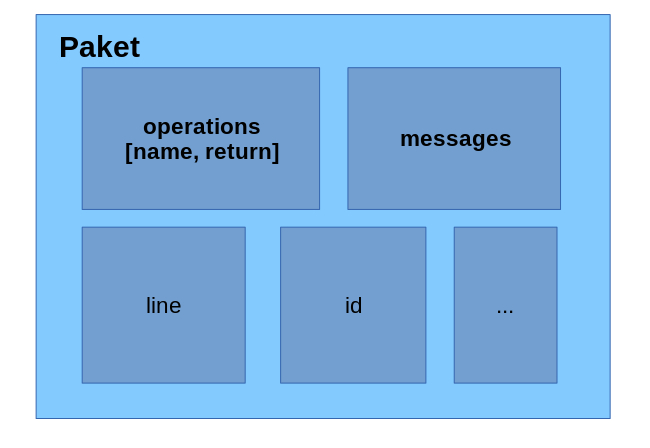
\includegraphics[scale=0.5]{simulation/Pakete2.jpg}
	\end{center}
	%Wir stellen verschiedene Paketschlüssel zur verfügung, am wichtigsten für die Simulation ist message und operations. Über Operations werden Funktionen beim Client aufgerufen und mit Message werden Nachrichten an den User übergeben. Bei look würden wir zb. ein operation-Paketelement erstellen mit name= look und return = zu highlightende Koordinate und nicht Element an dieser Koordinate -> das wird nicht benötigt.
\end{frame}
\subsection{Javascript-Client}

\begin{frame}
\begin{center}
	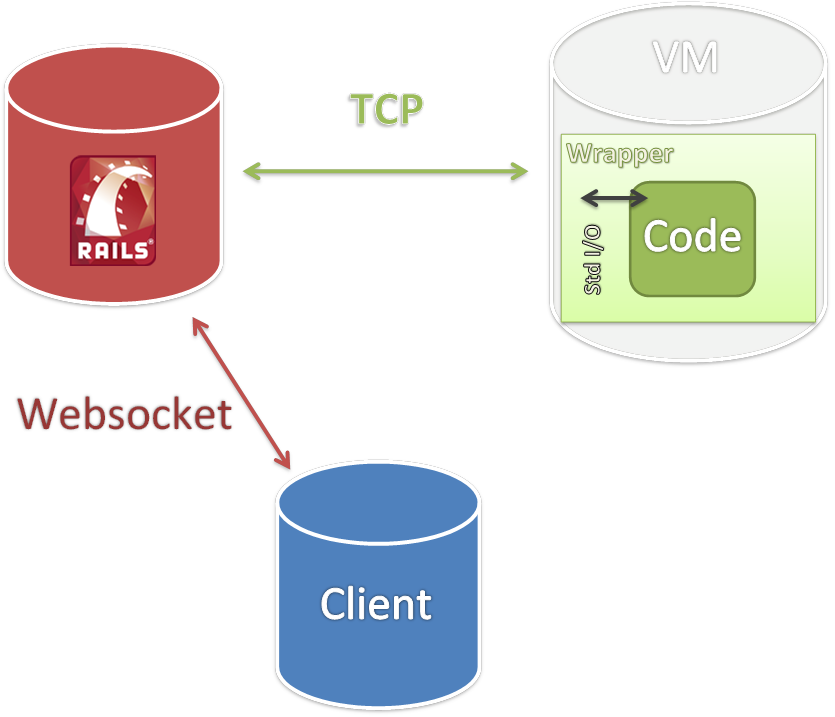
\includegraphics[scale=0.35]{overview}
\end{center}
\end{frame}

\begin{frame}
\frametitle{Web-Technologien}
\begin{center}
	
\includegraphics[scale=0.2]{client/HTML5_Logo.png}
	
\includegraphics[scale=0.2]{client/css3logo.png}
	
\end{center}		
	
	
	
\includegraphics[scale=0.4]{client/coffeescript-logo.png}
	
\includegraphics[scale=0.40]{client/less-logo.png}
	
\includegraphics[scale=0.045]{client/bootstrap-logo.png}
\end{frame}

\begin{frame}
\frametitle{Javascript-Client}
\begin{center}
	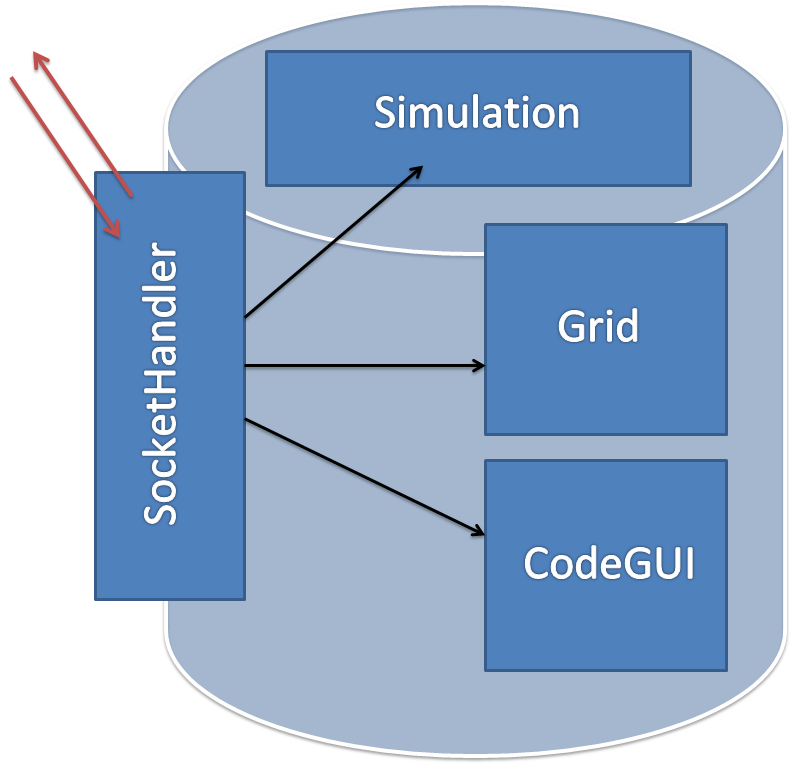
\includegraphics[scale=0.3]{client/modules.png}
\end{center}
\end{frame}


\begin{frame}
\frametitle{SocketHandler}
\inputminted[linenos, numbersep=2pt, tabsize=4, frame=lines, label=Beispiel Paket]{json}{client/packet.json}
\end{frame}

\begin{frame}
\frametitle{SocketHandler}
	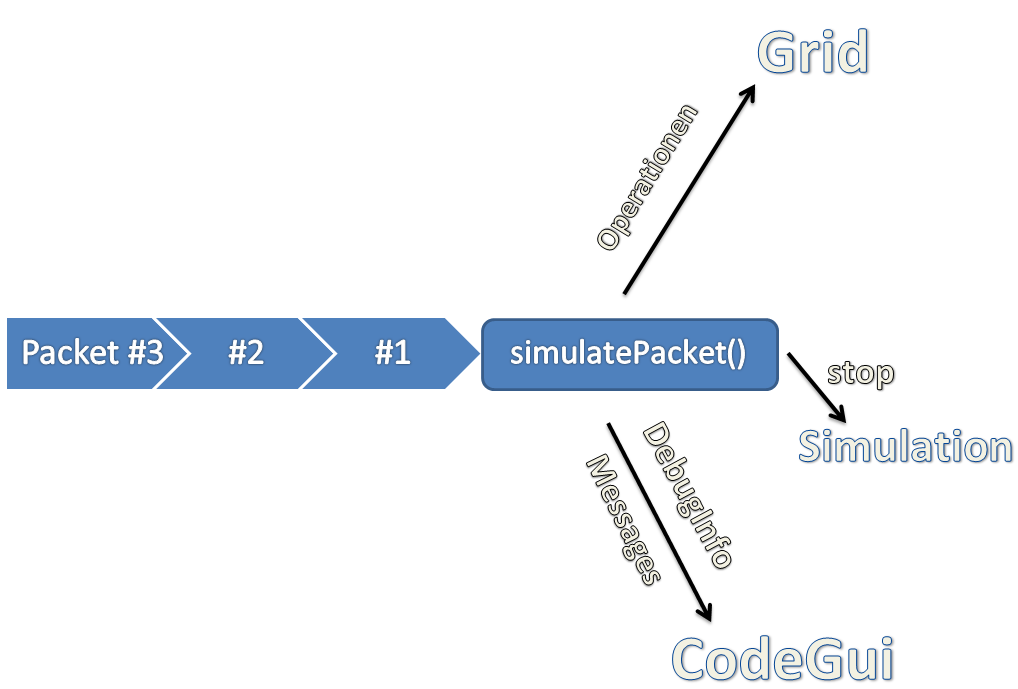
\includegraphics[scale=0.37]{client/socket-queue.PNG}
\end{frame}

\begin{frame}
\frametitle{CodeGUI}
\begin{center}
	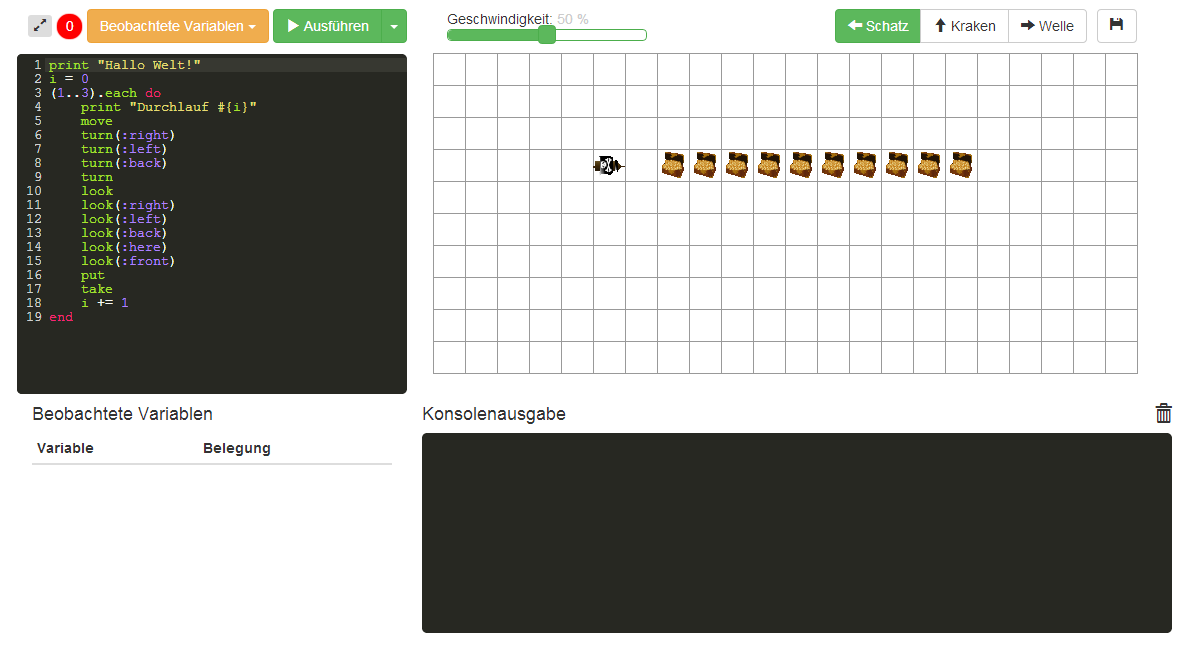
\includegraphics[scale=0.35]{client/client}
\end{center}
\end{frame}

\begin{frame}
\frametitle{Grid}
\begin{center}
	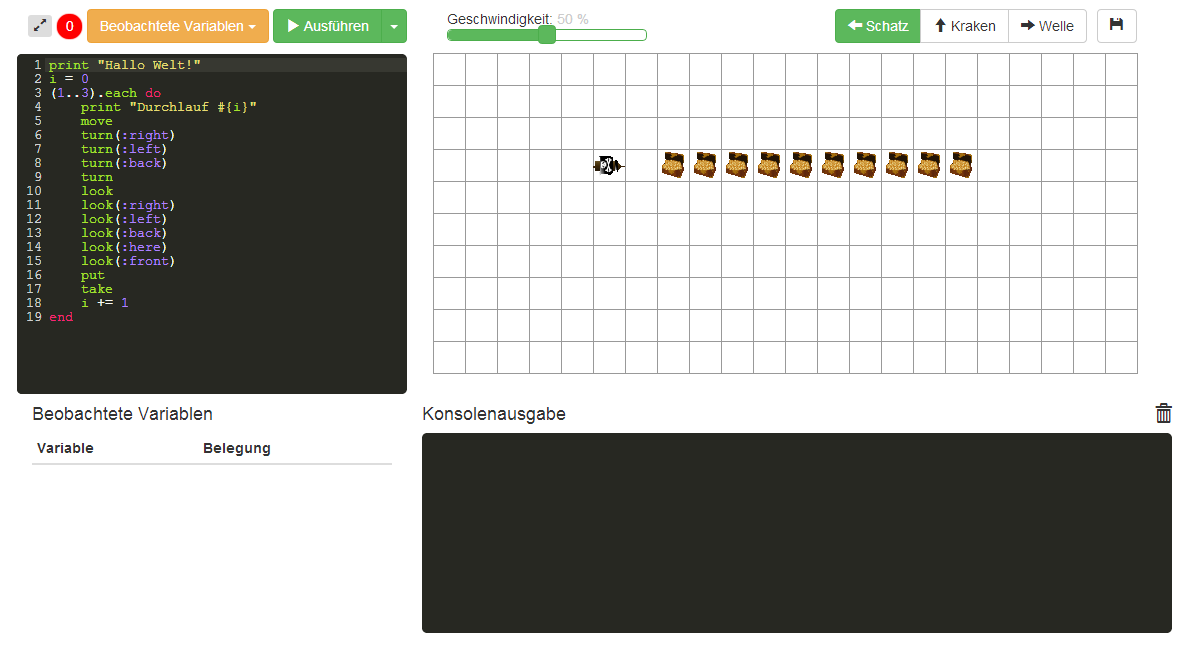
\includegraphics[scale=0.35]{client/client} %TODO
\end{center}
\end{frame}


\section{Individuelle Arbeiten}

\section{Präprozessor für Erlang}

\begin{frame}
Erlang
\end{frame}
\subsection{Scopes}




\begin{frame}
	\begin{itemize}
		\item[]\textbf{Komfortables Debuggen} \\
		\item[]	Einfügen der Jumpfunktion\\
		setzen von Breakpoints\\ 	
	\end{itemize}
	%Mein Thema ist die Einführung einer neuen Funktion.
\end{frame}

\begin{frame}
	\begin{center}
		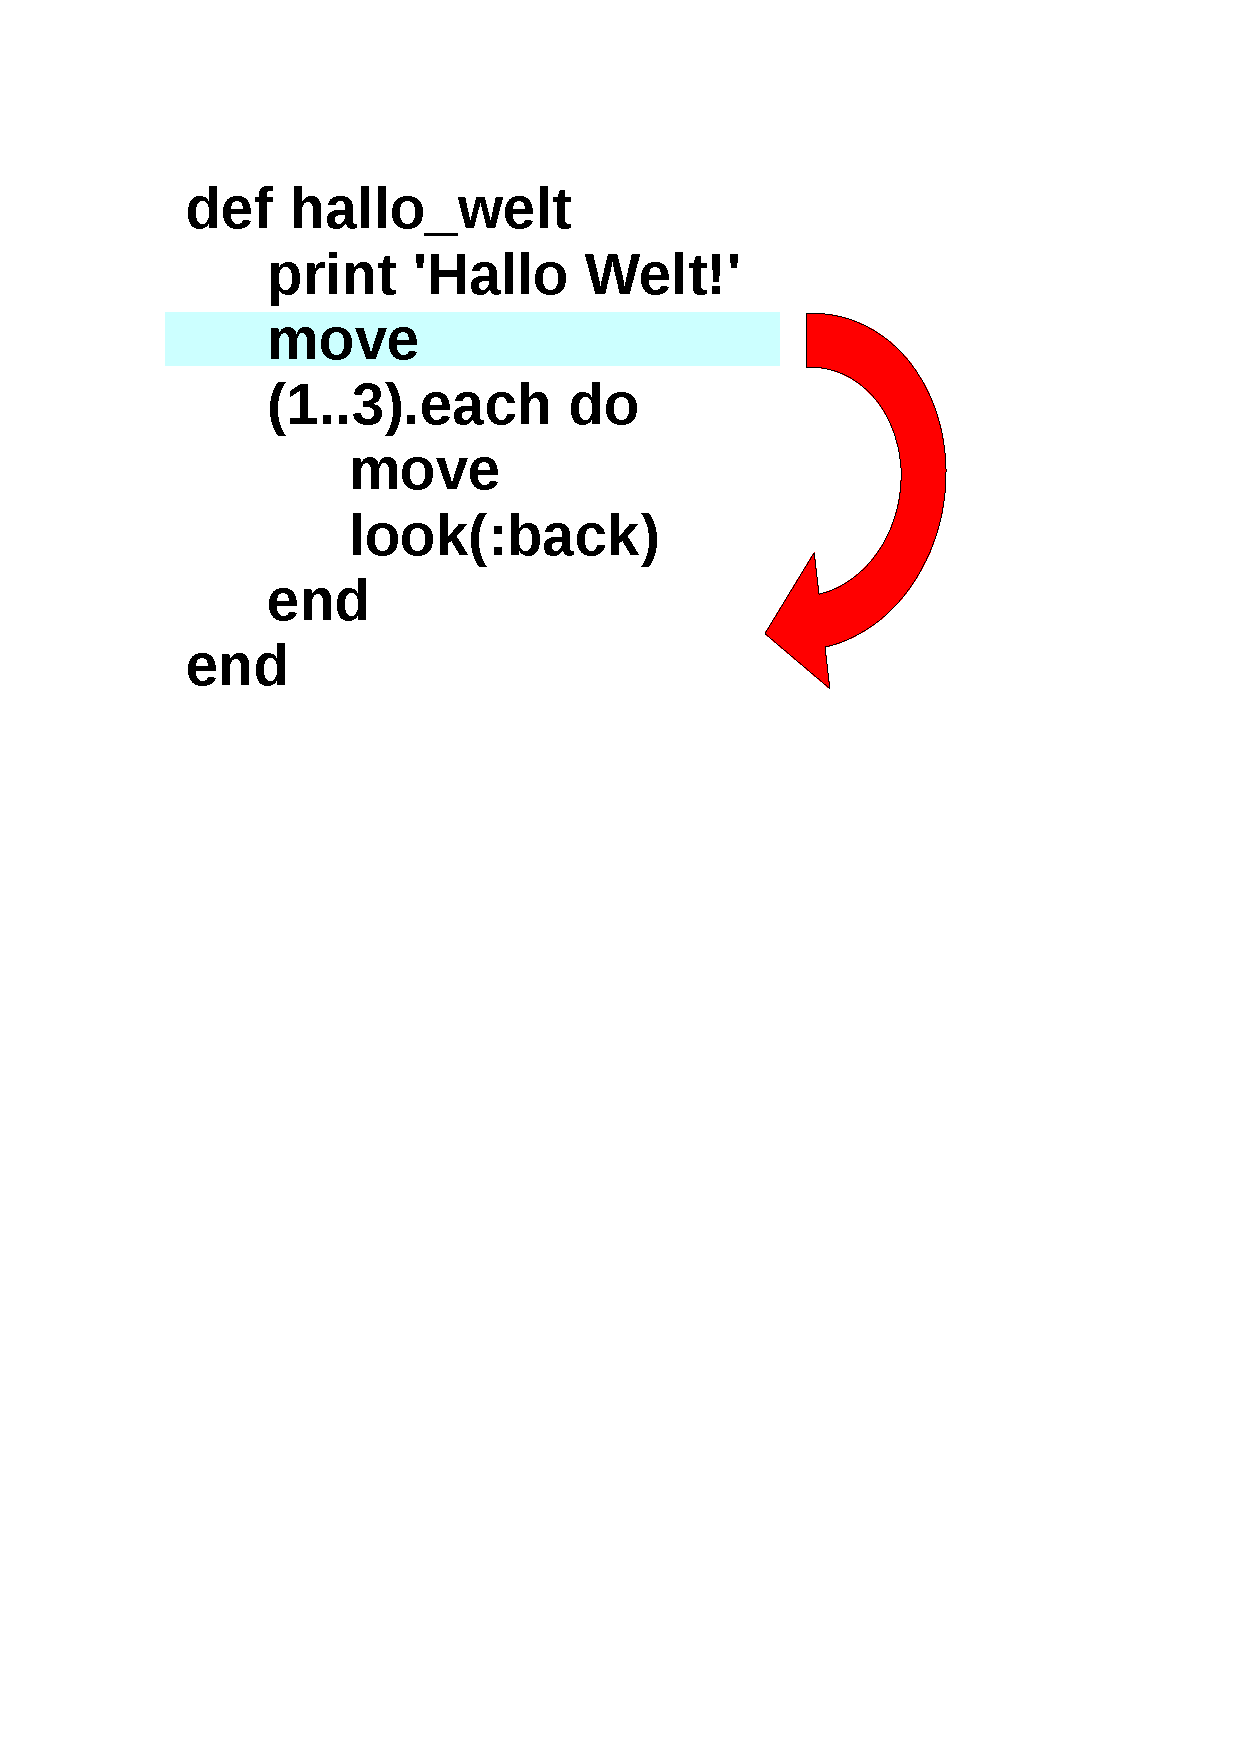
\includegraphics[scale=0.4]{scopes/Jump1.pdf}
	\end{center}
	% mit der "überspringen" Funktion soll man nicht nur Schrittweise durch den Text gehen können, sondern ganze Codeblöcke überspringen können. Zusätzlich soll die Möglichkeit bestehen, breakpoints zu setzten, bei denen eine normale Simulation anhält.
\end{frame}	

\begin{frame}

	\begin{center}
		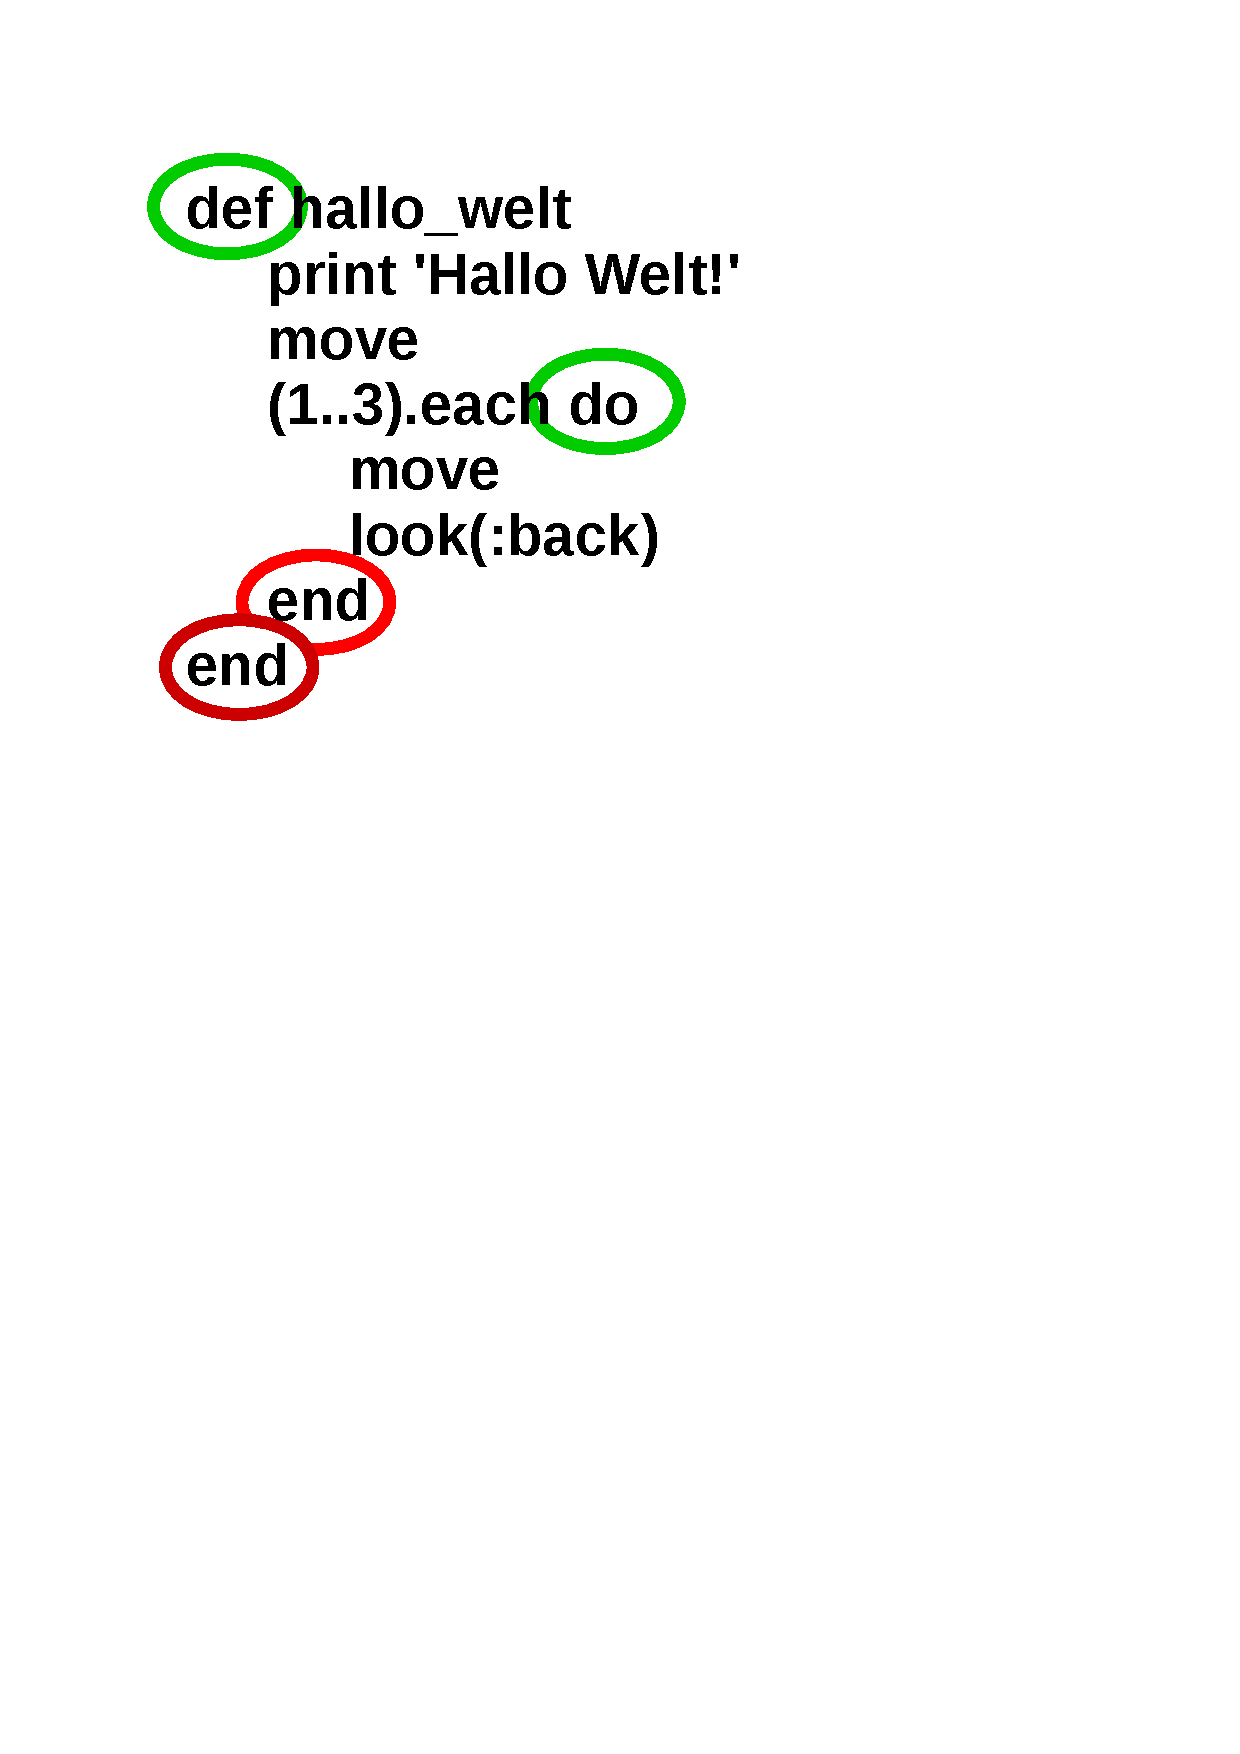
\includegraphics[scale=0.4]{scopes/beispiel2.pdf}
	\end{center}
	%Idee: Wir suchen nach Schlagwörtern im Text. 
\end{frame}

\begin{frame}
	\begin{center}
		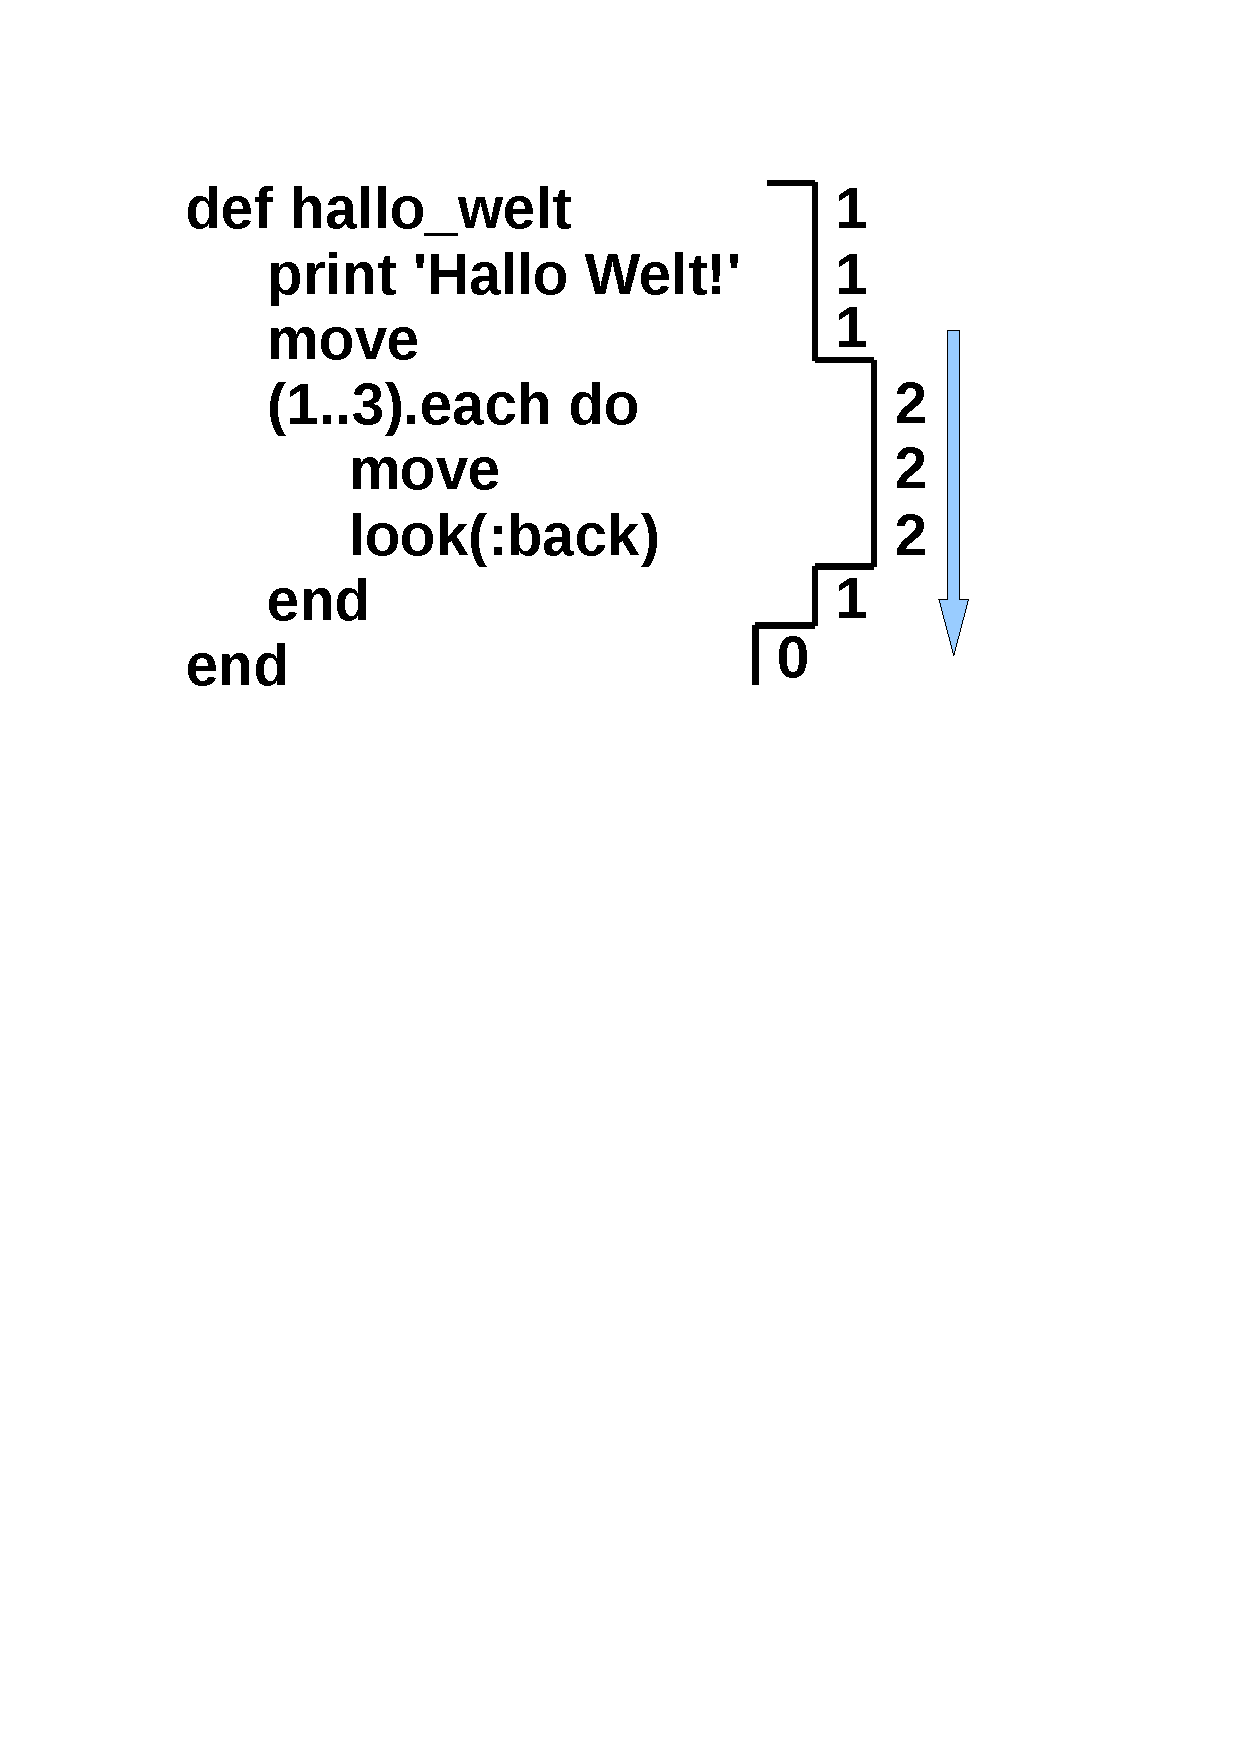
\includegraphics[scale=0.4]{scopes/beispiel3.pdf}
	\end{center}
	%Wird ein Blockanfang gefunden, gehen wir eine Ebene tiefer in den Laufzeitkeller (Stack). Wird das Ende eines Blockes erkannt, geht man wieder eine Ebene hinauf. Wenn man in der GUI die Funktion "Überspringen" auswählt, wird die Anfangstiefe gespeichert und es wird automatisch durch die Simulation gegangen, bis man an einem Punkt angelangt ist, wo die aktuelle Tiefe kleiner als die Anfangstiefe ist. Bei einer Anfangstiefe von 0 wird nur ein normaler Schritt durchgeführt.
\end{frame}

\begin{frame}

	\begin{itemize}
		\item[]\textbf{Schritt 1: Einfügen der $ break\_point $ Funktion} \\
		\item[]\textbf{Schritt 2: Automatische Blockerkennung und Einfügen der Funktion in den übergebenen Code} \\
	\end{itemize}
	%Was brauchen wir für den ersten Schritt:
\end{frame}

\begin{frame}
	\ \\
	\begin{center}
		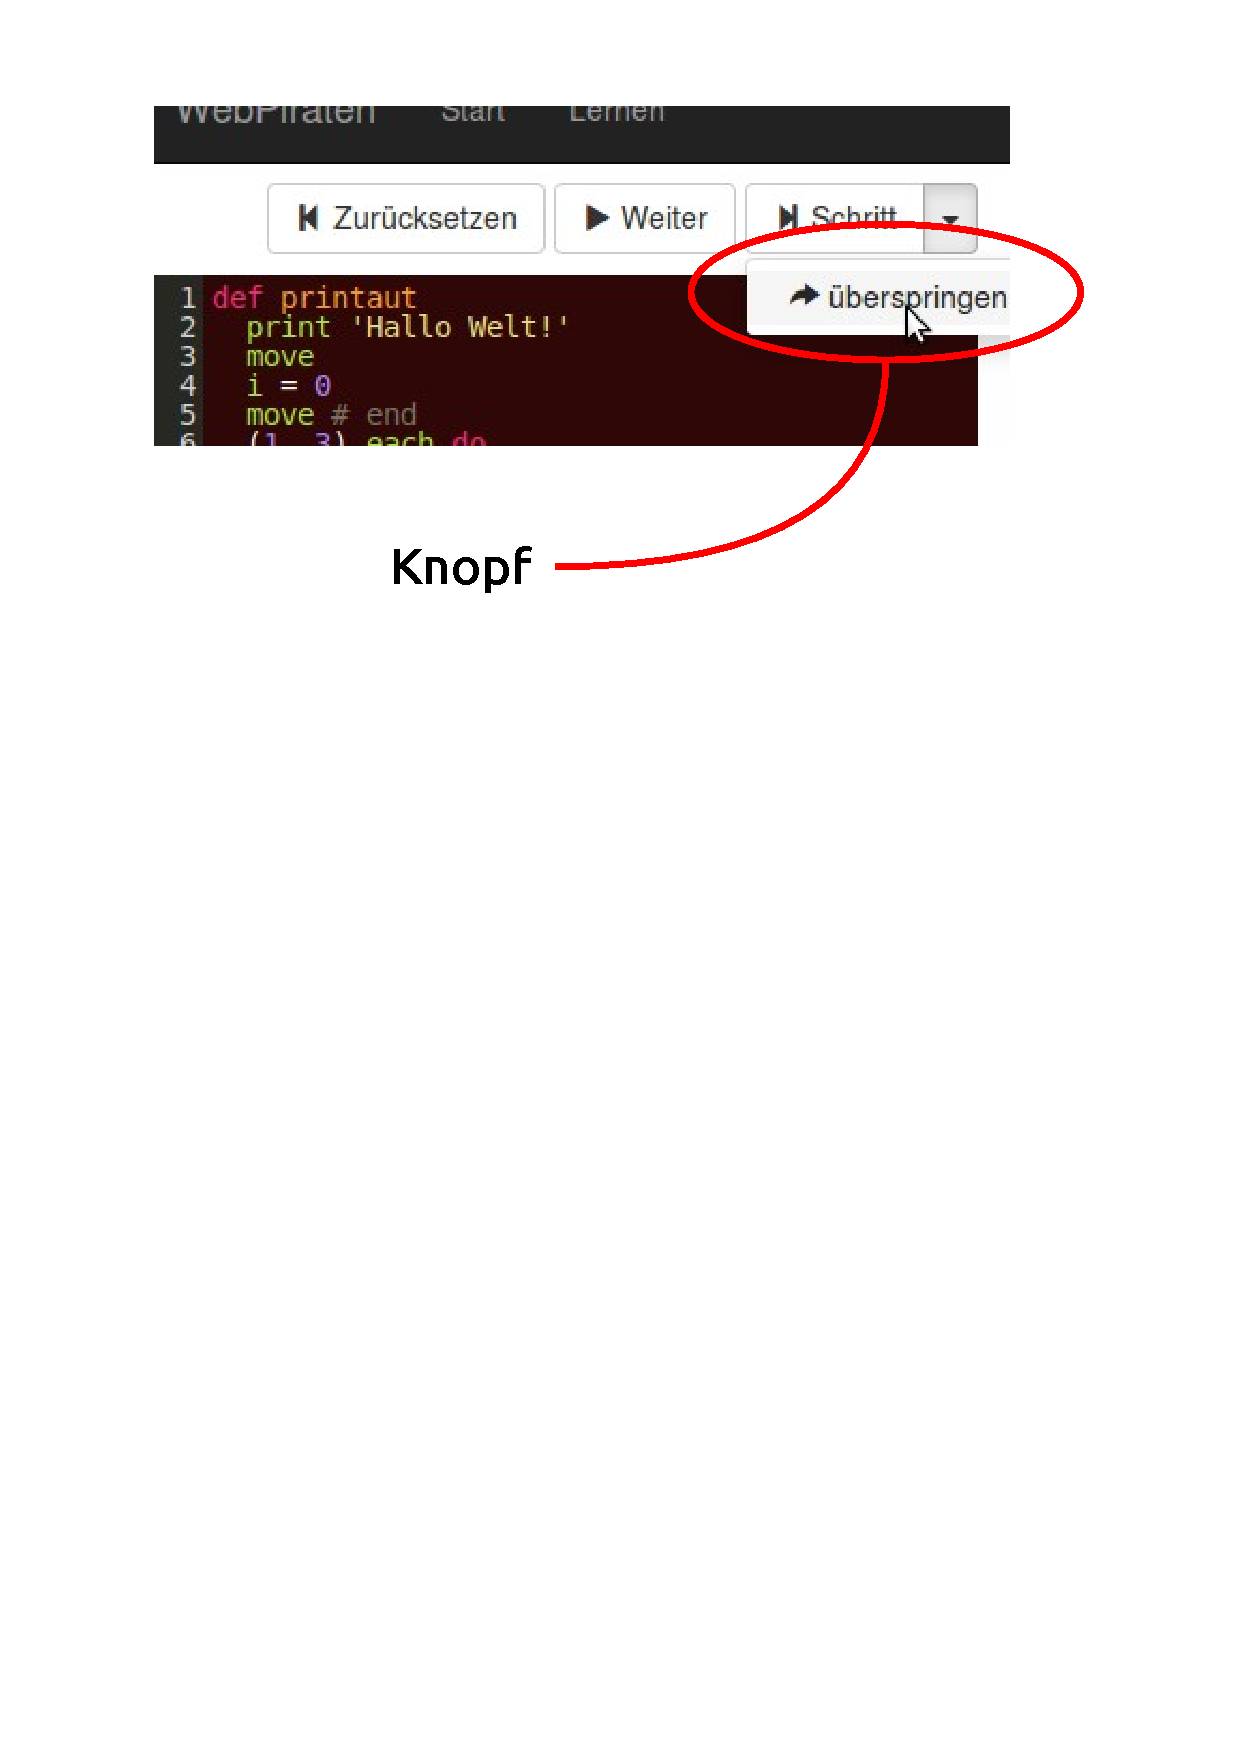
\includegraphics[scale=0.5]{scopes/button.pdf}
	\end{center}
	%Zuerst brauchen wir einen Button.
\end{frame}

\begin{frame}
	\begin{itemize}
		\item[]\textbf{Eine Funktion: $break\_point()$} \\
		\item[]\textbf{:point $\rightarrow$ Breakpoint} \\
		\item[]\textbf{:down $\rightarrow$ In den Keller} \\
		\item[]\textbf{:up \ \ $\rightarrow$ \ Aus dem Keller} \\
	\end{itemize}
	%Meine Lösung: die Funktion break\_ point(:arg) mit den Argumenten :
	%:point -> Breakpoint
	%:down -> erhöhung des Scopes
	%up -> verringerung des Scopes
\end{frame}

\begin{frame}
	\ \\
	\begin{center}
		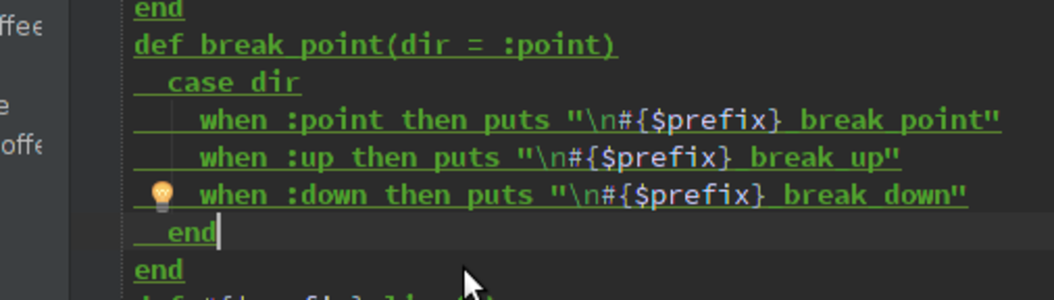
\includegraphics[scale=0.6]{scopes/preprocessor.pdf}
	\end{center}
	%Damit man eine Funktion im Code benutzen kann, müssen wir sie im Preprozessor vordefinieren. Wenn die VM den Code ausführt, soll sie die breakfunktion mit dem ausgesuchten parapeter aufrufen. 
\end{frame}

\begin{frame}
	\inputminted[linenos, frame=lines, label=rubyfunction]{ruby}{scopes/first.rb}
	%Die Breakfunktion packt einfach das Argument in das aktuelle Paket. Hierzu habe ich einen neuen Paket-Schlüssel definiert: :break (break ist vorgefiniert, deswegen heißt die Funktion break!) 
\end{frame}

\begin{frame}
	\begin{center}
		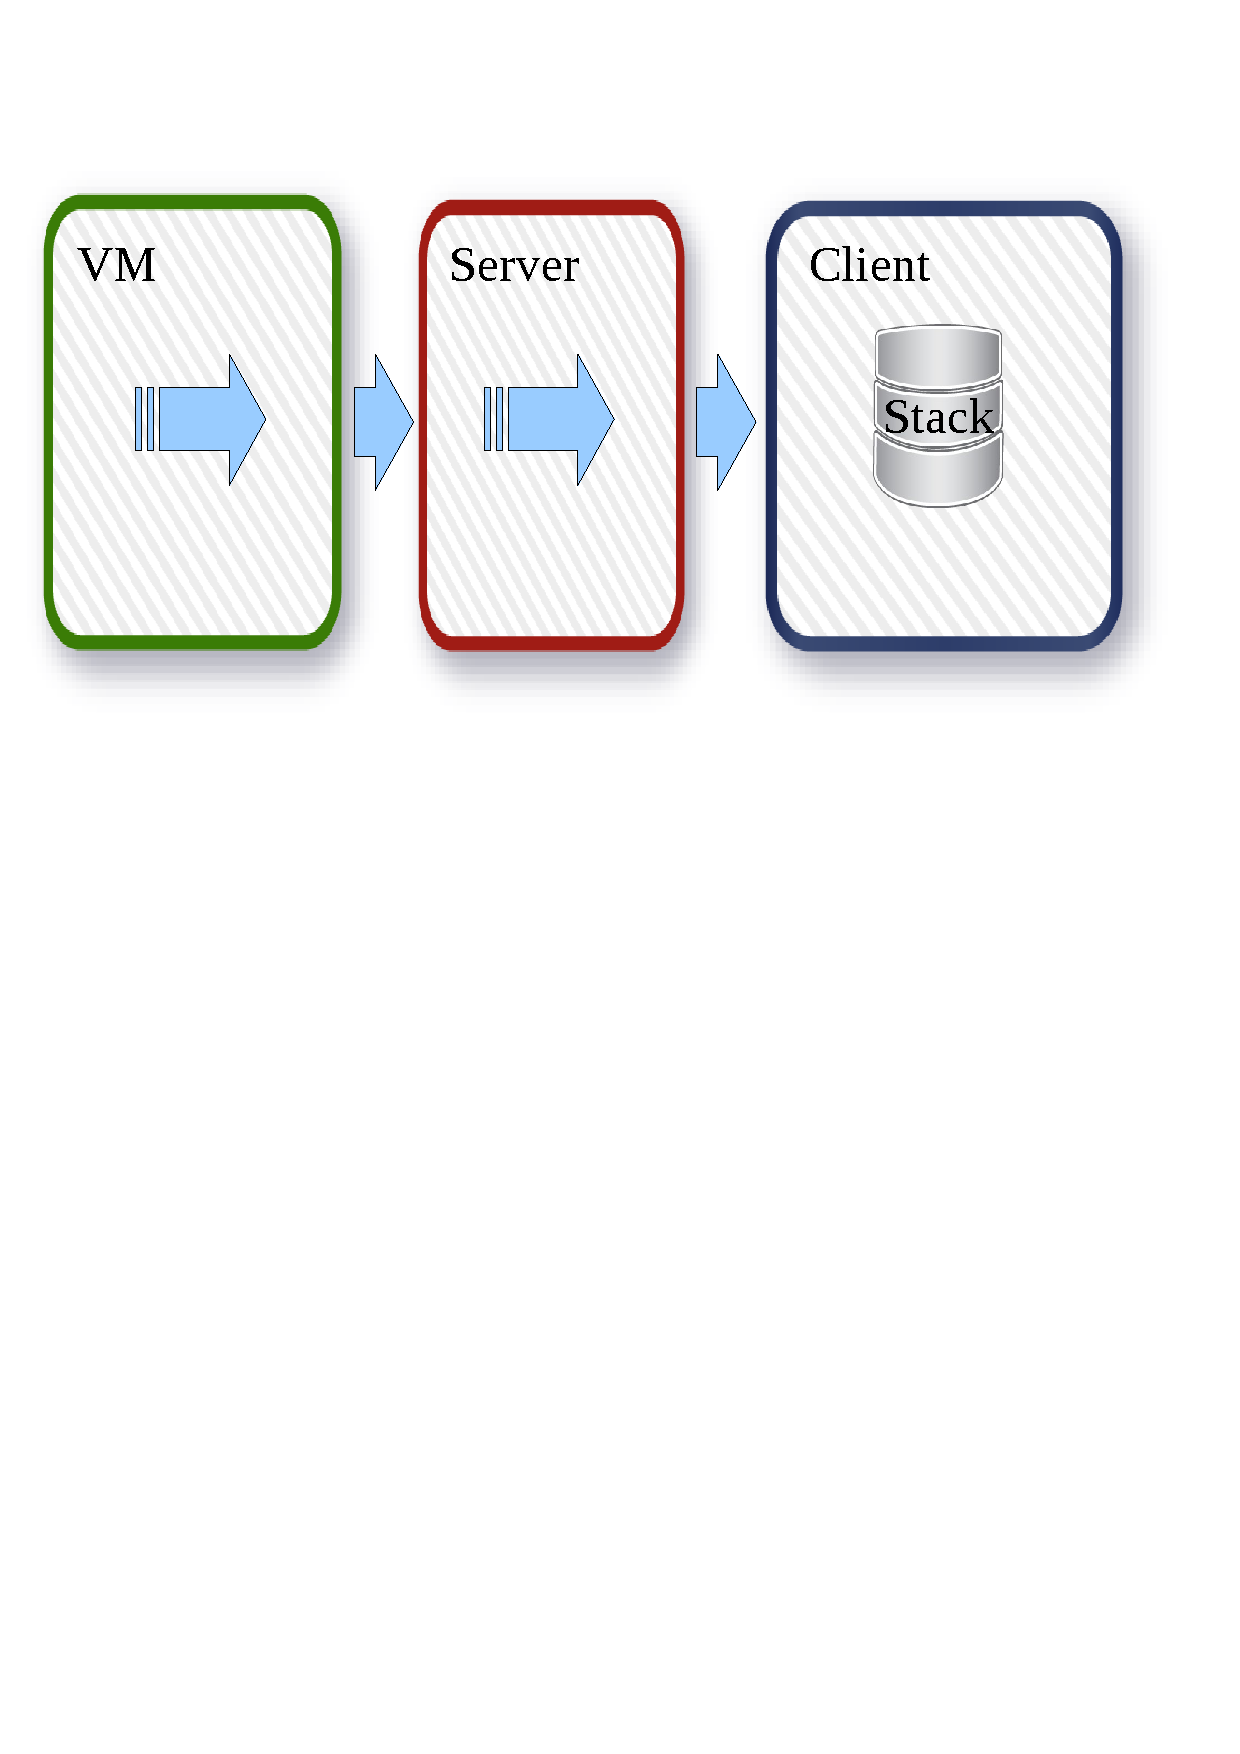
\includegraphics[scale=0.5]{scopes/stacks.pdf}
	\end{center}
	%Die VM und der Server geben also nur die Argumente an den Client weiter, wo ich eine Variable Stackdeep angelegt hab. Kommt ein Packet mit einem :break Element an, wird nur die Variable hoch oder runter gezählt.
	%Wenn man "überspringen" auswählt, wird die Stack deep gespeichert und die Pakete solange simuliert, bis die Stackdeep kleiner als der gespeicherte Wert ist. 
	%Wenn in einem Paket ein Breakpoint gesetzt werden soll, rufen wir einfach dir Funktion Simulation.stop() auf, die auch ausgeführt wird, wenn man auf den Stop Button drück.
\end{frame}

\begin{frame}
	\begin{itemize}
		\item[]\textbf{Automatische Blockerkennung} \\
		\item[]\textbf{Beispiel: Ruby} \\
	\end{itemize}
	%Jetzt also die automatische Blockerkennung. Als Beispielsprache nehme ich nun Ruby. Die automatische Blockerkennung ist Sprachenabhänging und muss für jede Sprache einzeln programiert werden. 
\end{frame}

\begin{frame}
	\begin{center}
		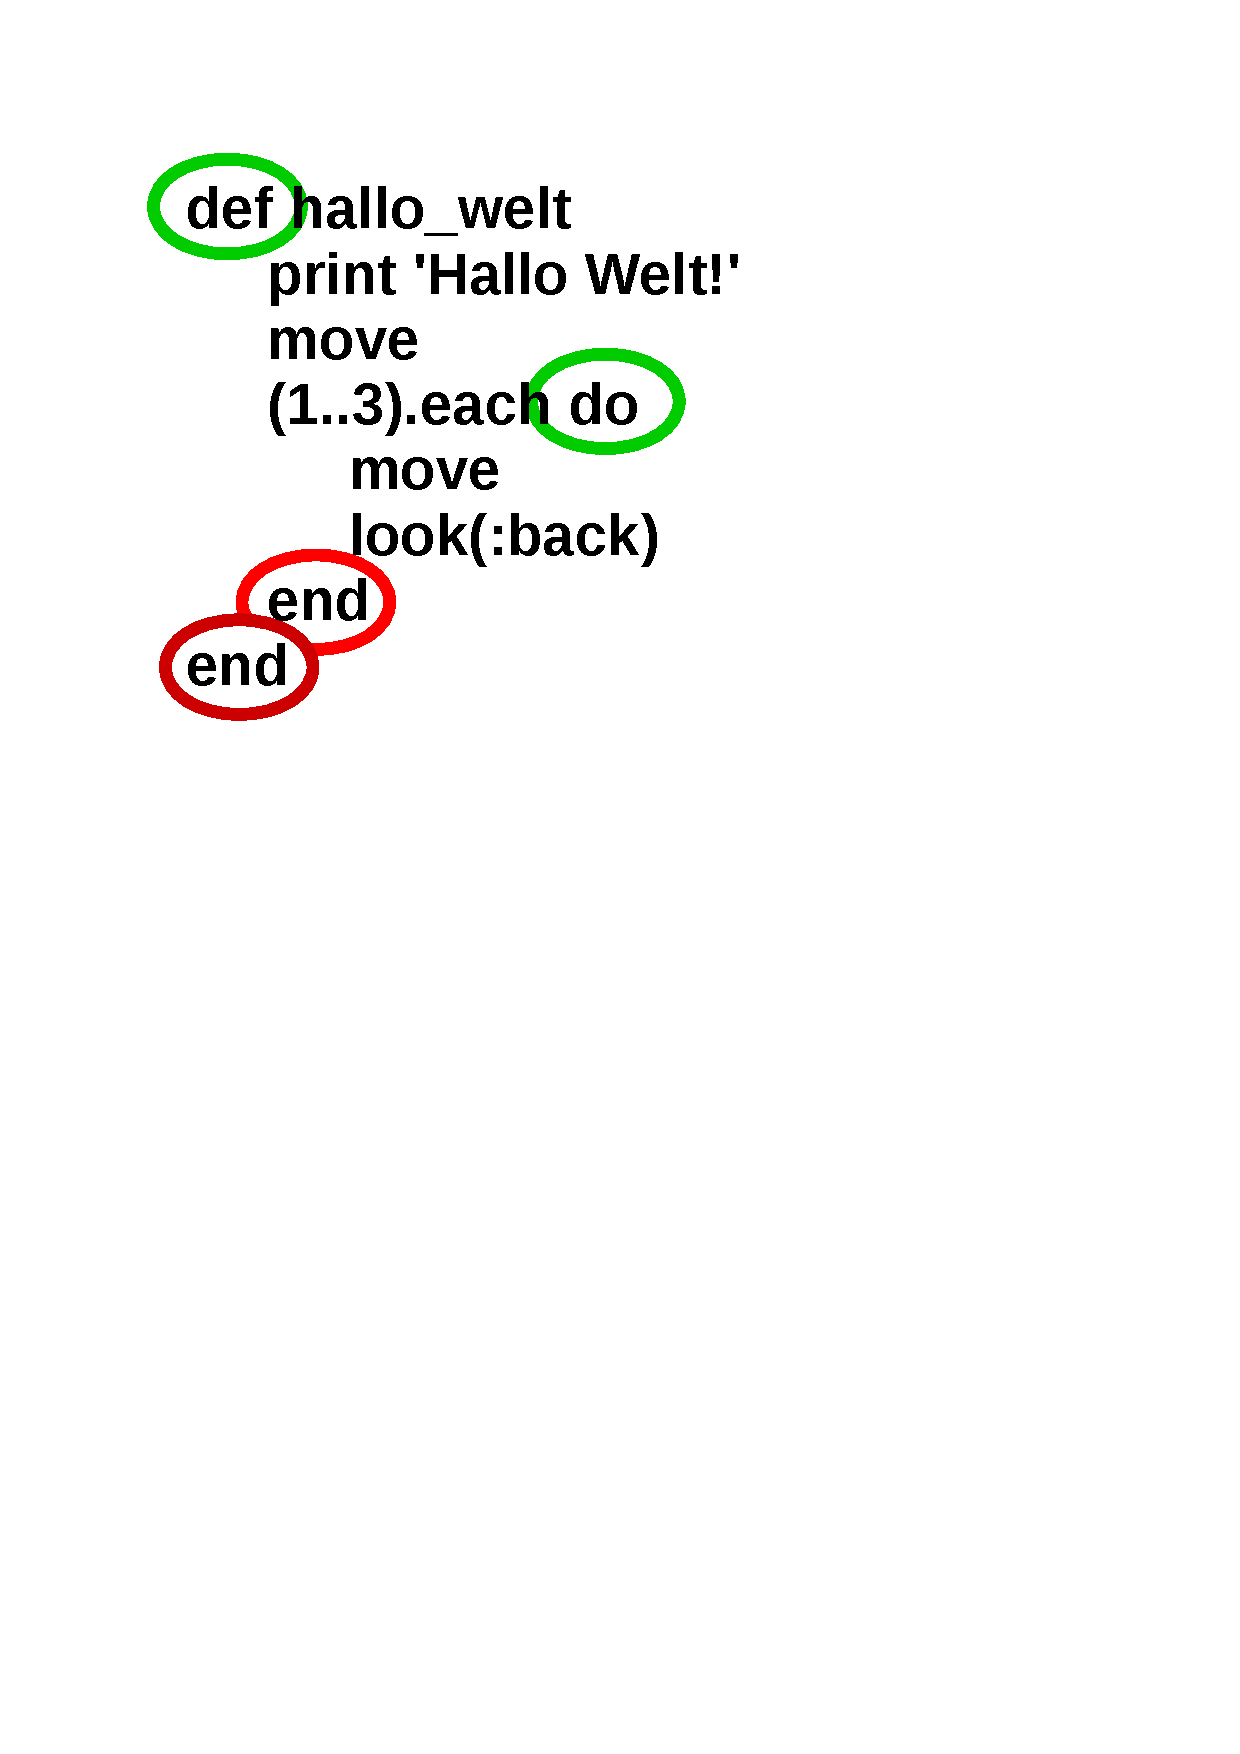
\includegraphics[scale=0.4]{scopes/beispiel2.pdf}
	\end{center}
	%Ich will die Blöcke erkennen, die mit 'end' beendet werden, also hab ich in einer Liste von Schlagwörtern für Ruby alle relevanten rausgeschrieben.
\end{frame}

\begin{frame}
	\begin{itemize}
		\item[]\textbf{class\\ def\\ module\\ if (unless)\\ while\\ for\\ until\\ do\\ case\\ begin\\ BEGIN\\ END\\}
	\end{itemize}
	%Die Liste ist dann doch etwas länger geworden.
\end{frame}

\begin{frame}
	\begin{center}
	\ \\
		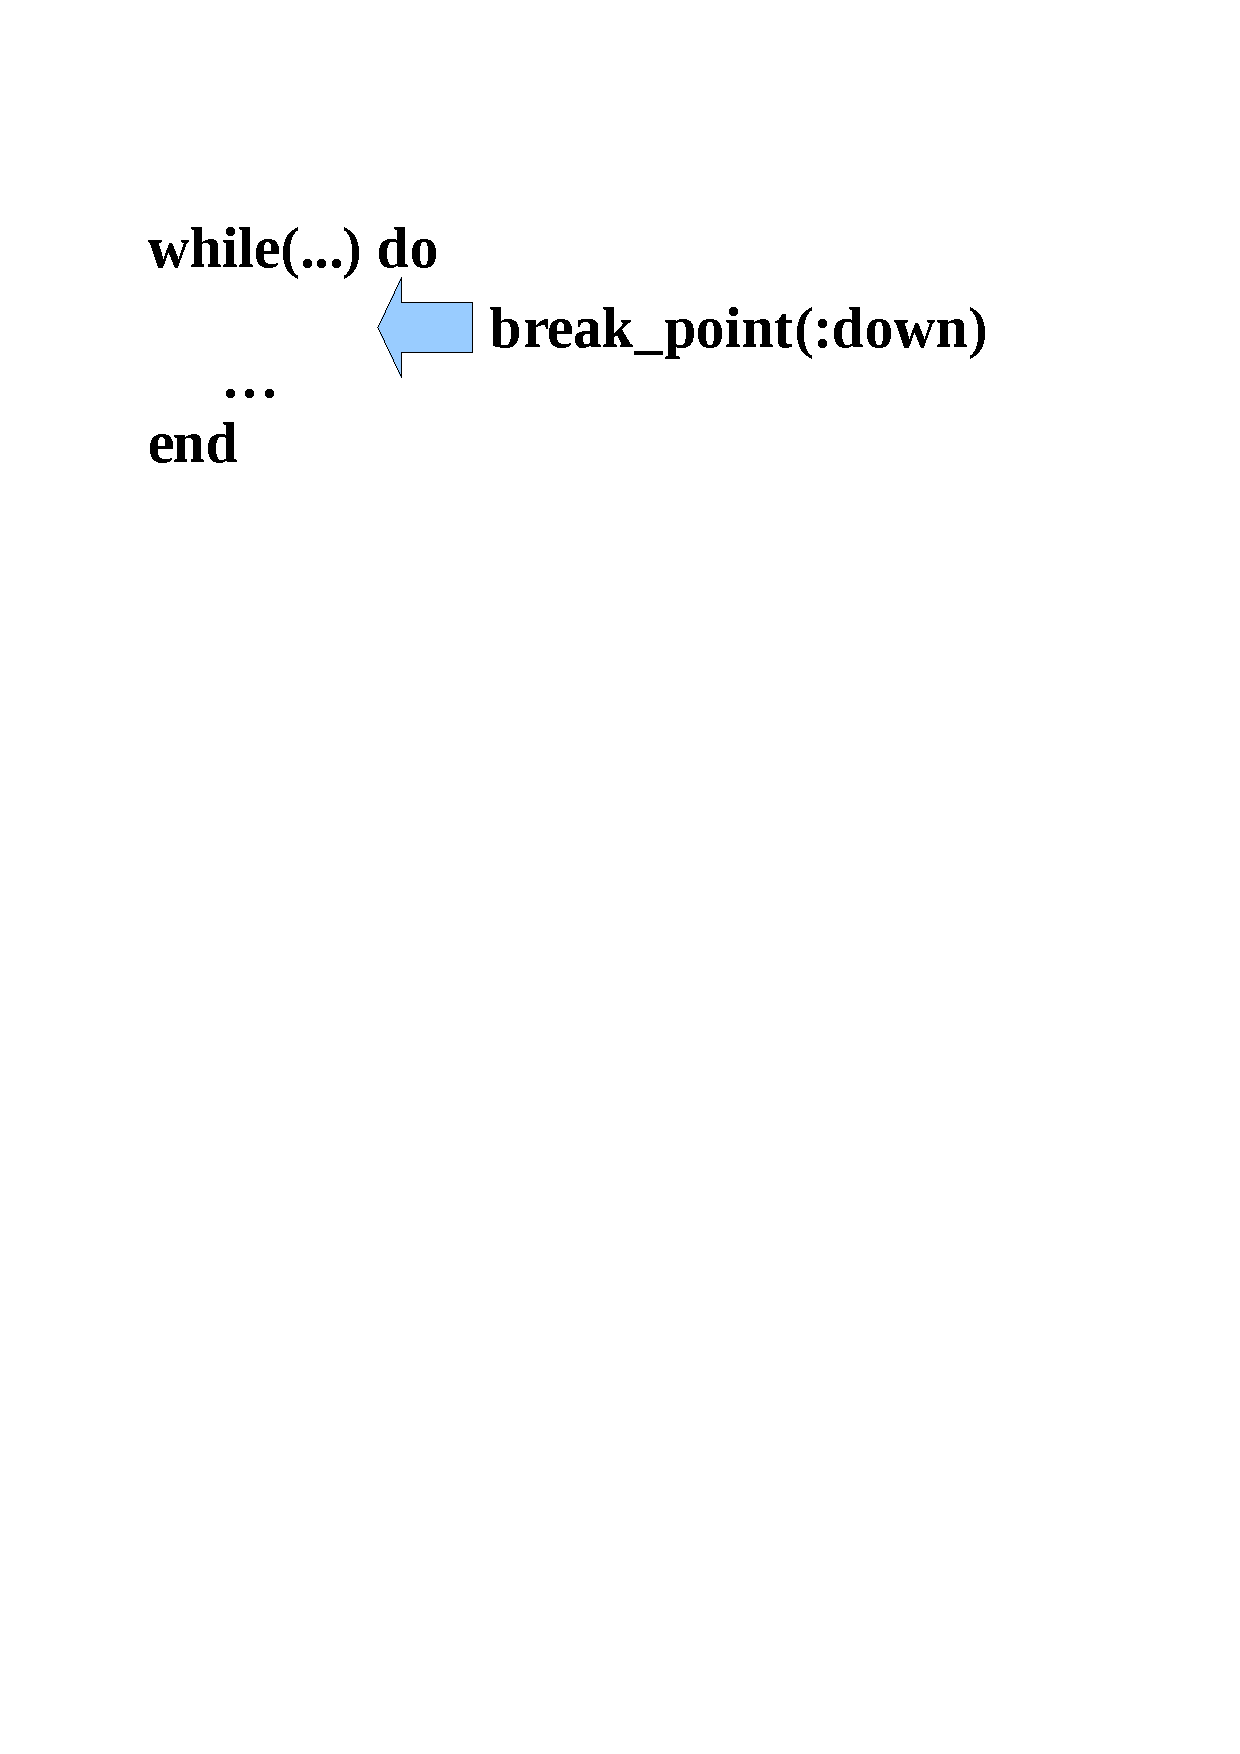
\includegraphics[scale=0.4]{scopes/beispiel4.pdf}
	\end{center}
	%Es stellt sich also die Frage, wo ich die Funktion in den Code einfügen möchte. Zuerst dachte ich, direkt nach dem Schlüsselwort, bei einer Schleife würden wir dann jedoch immer wieder die Funktion aufrufen.
\end{frame}

\begin{frame}
	\begin{center}
		\ \\ \ \\
		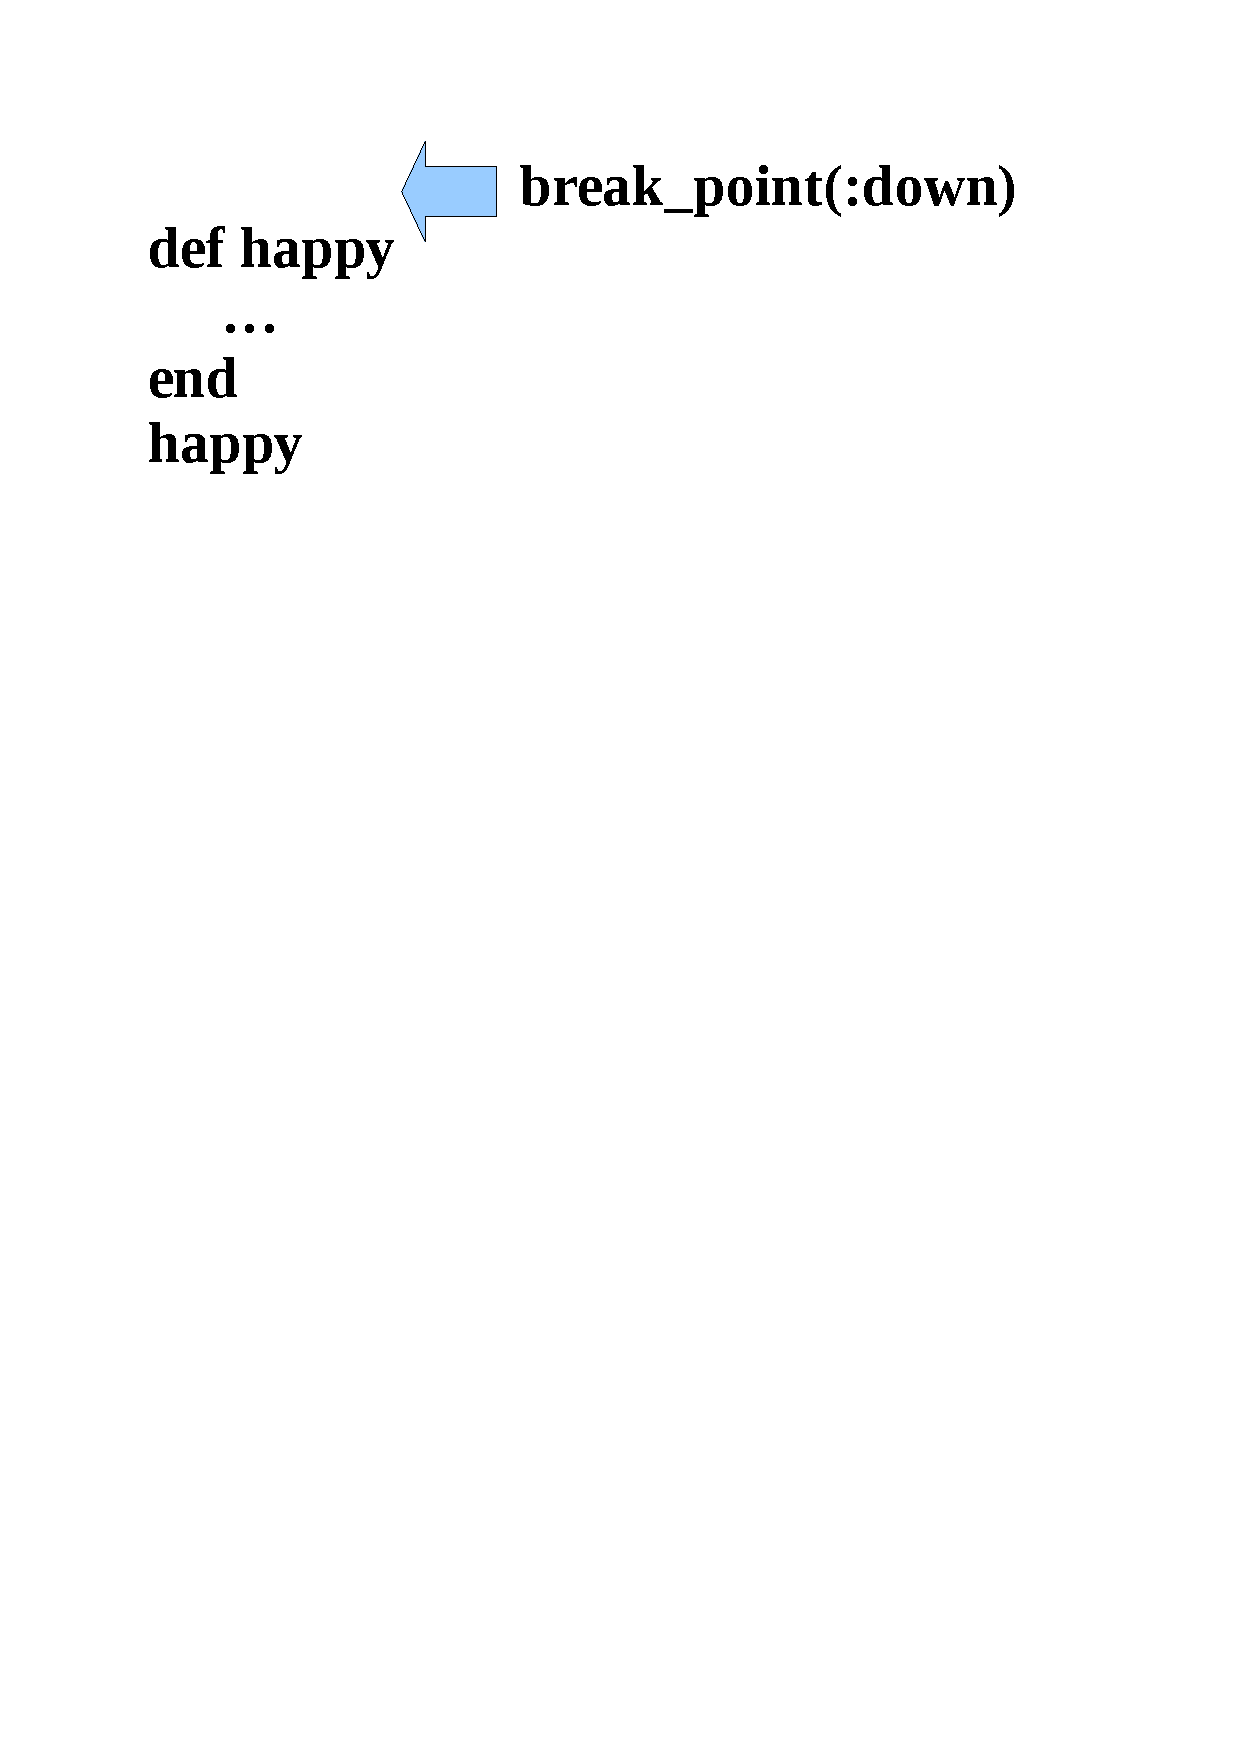
\includegraphics[scale=0.4]{scopes/beispiel5.pdf}
	\end{center}
	%Also dachte ich, direkt in der Zeile vor dem Schlüsselwort. Definiert man aber eine Funktion und ruft diese später auf, wird die Zeile vor der Funktion natürlich nicht ausgeführt. Also musste ich meine List unterteilen.
\end{frame}

\begin{frame}
	\begin{center}
		\begin{tabular}{c|c}
			\textbf{Vor} & \textbf{Hinter} \\ 
			\hline 
			\textbf{for} & \textbf{def} \\ 
			\textbf{until} & \textbf{class} \\
			\textbf{while} & \textbf{module} \\
			\textbf{if/unless} & \textbf{BEGIN} \\
			\textbf{do} & \textbf{END} \\
			\textbf{case} &  \\
		\end{tabular}
	\end{center}
	%bei den Operatoren, bei denne ich die break_down Funktion vor dem Öffnen des Blocks setzt, setzt ich die break_up Funktion hinter das dazugehörige end. Für die unterscheidung der ends benutzte ich eine Liste, zu der ich bei jedem öffnen eines Blockes ein passendes Element hinzufüge und beim schließen das zuletzt hinzugefügte Element untersuche und lösche.
	%da durch return eine Funktion vorzeitig beendet werden kann, muss man auch vor einem return die break Funktion aufrufen.
	%Ein weiteres Problem ist, dass z.B. bei der While Schleife zusätzlich zu dem while ein do gesetzt werden kann. Zur Zeit prüfe ich den Code zuerst auf die Schlüsselwörter, auf die optimal auch ein do folgen kann und erst wenn keines dieser Wörter gefunden wurde prüfe ich auf do.
\end{frame}

\begin{frame}
	\inputminted[linenos, frame=lines, label=Beispiel]{ruby}{scopes/beispiel.rb}
	%Weitere Fälle müssen untersucht werden: Kommentare und String. Schlüsselwörter, die in solchen Bereichen stehen, müssen ignoriert werden. Und man muss aufpassen, dass man die breakfunktion nicht ausversehen in einen Kommentar oder string einfügt.
	%Zur Zeit suche ich mit der index Funktion nach Kommentaren. Sie liefert die Stelle, an dem ein Zeichen das erste mal vorkommt. Genau davor würde ich dann die Funktion kopieren.
\end{frame}

\begin{frame}
	\begin{itemize}
		\item[]\textbf{Momentane Einschränkungen:}
		\item[]Nur eine break- Funktion pro Zeile
		\item[]Keine Schlagwörter in Strings
		\item[]Keine break- Funktionen in Zeilen mit multiline Strings
		\item[]\textbf{...}
	\end{itemize}
	%Bis jetzt muss man sich an die folgenden Bedingungen halten, damit die Jump Funktion korrekt genutzt werden kann... Da ich noch nicht fertig bin, werden mir bestimmt in den nächsten Wochen weitere Probleme auffallen. In der nächsten Zeit werde ich versuchen, diese Probleme möglichst zu beheben. Idee zu Strings: Codezeile kürzen und gekürzte Zeile überprüfen.
\end{frame}

\subsection{Sicherheit}

\begin{frame}
\frametitle{SQL-Injection}
\end{frame}

\begin{frame}
\frametitle{Cross-Site-Scripting}

\end{frame}

\begin{frame}
\frametitle{Aufbau der VM}
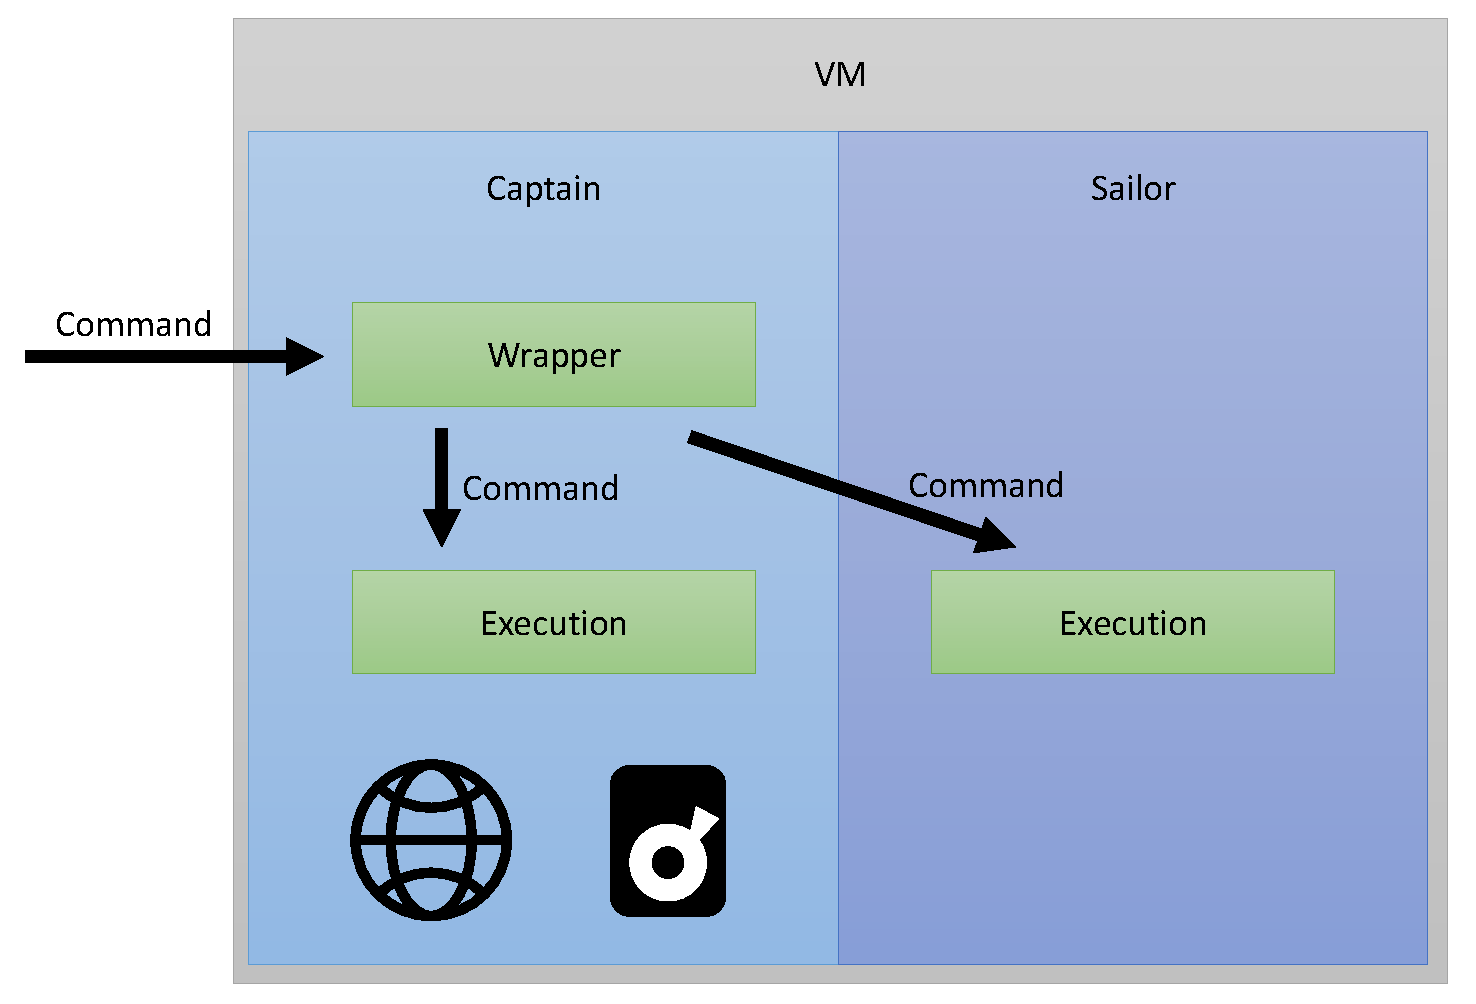
\includegraphics[width=300pt]{security/user.pdf}

\end{frame}
\subsection{Performance}

\begin{frame}
wroooooooooooooooooooom!!!
\end{frame}

\begin{frame}
\frametitle{Bildquellen}
\begin{itemize}
	\item \url{rubyonrails.org}
	\item \url{commons.wikimedia.org/wiki/File:Stoppuhr_hanhart.jpg}
	\item \url{logonoid.com/bootstrap-logo}
	\item \url{lesscss.org}
	\item \url{coffeescript.org}
	\item HTML5 \& CSS3 Logo:\url{ w3c.org}
	\item \url{erlang.org}
	\item \url{http://commons.wikimedia.org/wiki/File\%3AVerbotsschild.svg}
\end{itemize}
\end{frame}

\end{document}